% \documentclass[twoside,11pt,openright]{report}
\documentclass[ twoside,openright,titlepage,numbers=noenddot,headinclude,%1headlines,% letterpaper a4paper
                footinclude=true,cleardoublepage=empty,abstractoff, % <--- obsolete, remove (todo)
                BCOR=5mm,paper=a4,fontsize=11pt,%11pt,a4paper,%
                ngerman,english,%
                ]{scrreprt}
\PassOptionsToPackage{eulerchapternumbers,listings,
                      pdfspacing,%floatperchapter,
                      % linedheaders,%
                      subfig,beramono
                      % ,eulermath
                    }{classicthesis}
\usepackage{classicthesis}

\usepackage[left=1.7in,right=1.2in,top=1in,bottom=1in]{geometry}% \setlength{\marginparwidth}{1em}%

\usepackage{textcomp} % fix warning with missing font shapes
\usepackage{scrhack} % fix warnings when using KOMA with listings package
\usepackage{xspace} % to get the spacing after macros right
\usepackage{mparhack} % get marginpar right
\usepackage{fixltx2e} % fixes some LaTeX stuff --> since 2015 in the LaTeX kernel (see below)

\usepackage[latin1]{inputenc}
\usepackage[T1]{fontenc}
\usepackage[american]{babel}
% \usepackage{a4}
\usepackage{latexsym}
\usepackage{amssymb}
\usepackage{amsmath}
\usepackage{mathtools}
\usepackage{epsfig}
\usepackage{mathptmx}
\usepackage{color}
\usepackage{epstopdf}
% \usepackage{microtype}
\usepackage{hyperref}
\usepackage[square,numbers,sort&compress]{natbib}
\usepackage[useregional]{datetime2}
\DTMlangsetup[en-US]{showdayofmonth=false}
% \usepackage{lipsum}
% \usepackage{listings}
\usepackage{tikz}
\usepackage{lstautogobble}
\usepackage{subcaption}

\usepackage{amsthm}                                % Theorem package
\theoremstyle{definition}                          % plain, definition, remark
\renewcommand*{\proofname}{Proof}


\renewcommand*\sfdefault{lmss}
\renewcommand*\ttdefault{txtt}
\newcommand{\easycrypt}{\texttt{EasyCrypt}}
\newcommand{\validviews}[1]{\textbf{Valid}$(#1)$}
\newcommand{\indis}[1]{=\{#1\}}
\newenvironment{draft}{\color{red}}{\ignorespacesafterend}

\newtheorem{theorem}{Theorem}[section]
\newtheorem{lemma}[theorem]{Lemma}
\newtheorem{proposition}[theorem]{Proposition}
\newtheorem{corollary}[theorem]{Corollary}
\newtheorem{definition}[theorem]{Definition}
\newtheorem{conjecture}[theorem]{Conjecture}

\newcommand{\ie}{i.\,e.}
\newcommand{\Ie}{I.\,e.}
\newcommand{\eg}{e.\,g.}
\newcommand{\Eg}{E.\,g.}

\newcommand{\todo}[1]{{\color[rgb]{.5,0,0}\textbf{$\blacktriangleright$#1$\blacktriangleleft$}}}

\newcommand{\decomp}{\mathcal{D}}
\newcommand{\view}{\textbf{w}}
\newcommand{\tape}{\textbf{k}}
\DeclarePairedDelimiter{\Prfences}{[}{]}
\renewcommand{\Pr}{\operatorname{Pr}\Prfences}

\definecolor{mygreen}{rgb}{0,0.6,0}
\definecolor{mygray}{rgb}{0.5,0.5,0.5}
\definecolor{mymauve}{rgb}{0.58,0,0.82}

\lstset{
  morecomment=[s]{(*}{*)},
  morecomment=[n]{(*}{*)},
  keywordstyle=\color{RoyalBlue},%\bfseries,
  basicstyle=\small\ttfamily,
  commentstyle=\color{Green}\ttfamily,
  stringstyle=\rmfamily,
  numbers=none,%left,%
  numberstyle=\scriptsize,%\tiny
  stepnumber=5,
  numbersep=8pt,
  showstringspaces=false,
  breaklines=true,
  %frameround=ftff,
  belowcaptionskip=.75\baselineskip,
  %frame=L
  backgroundcolor=\color{white},   % choose the background color; you must add \usepackage{color} or \usepackage{xcolor}; should come as last argument
  breakatwhitespace=false,         % sets if automatic breaks should only happen at whitespace
  captionpos=b,                    % sets the caption-position to bottom
  deletekeywords={...},            % if you want to delete keywords from the given language
  escapeinside={\%*}{*)},          % if you want to add LaTeX within your code
  extendedchars=true,              % lets you use non-ASCII characters; for 8-bits encodings only, does not work with UTF-8
  % firstnumber=1000,                % start line enumeration with line 1000
  frame=single,	                   % adds a frame around the code
  keepspaces=true,                 % keeps spaces in text, useful for keeping indentation of code (possibly needs columns=flexible)
  % language=Octave,                 % the language of the code
  morekeywords={*,module,type,proc,Pr,equiv,hoare,lemma,forall, phoare,
    res,op,with,let,in,require,const,var,return,pred,None,Some,clone,export,as,realize,by,split},            % if you want to add more keywords to the set
  rulecolor=\color{black},         % if not set, the frame-color may be changed on line-breaks within not-black text (e.g. comments (green here))
  showspaces=false,                % show spaces everywhere adding particular underscores; it overrides 'showstringspaces'
  showtabs=false,                  % show tabs within strings adding particular underscores
  tabsize=2,	                   % sets default tabsize to 2 spaces
  % title=\lstname                   % show the filename of files included with
  % \lstinputlisting; also try caption instead of title
}

\begin{document}

%%%%%%%%%%%%%%%%%%%%%%%%%%%%%%%%%%%%%%%%%%%%%%%%%%%%%%%%%%%%%%%%%%%%%%%

\pagestyle{empty} 
\pagenumbering{roman} 
\vspace*{\fill}\noindent{\rule{\linewidth}{1mm}\\[4ex]
{\Huge\sf Formalising Sigma-Protocols and commitment schemes within \easycrypt}\\[2ex]
{\huge\sf Nikolaj Sidorenco, 201504729}\\[2ex]
\noindent\rule{\linewidth}{1mm}\\[4ex]
\noindent{\Large\sf Master's Thesis, Computer Science\\[1ex]
  \today \\[1ex] Advisor: Bas Spitters\\[1ex]
  Co-advisor: Sabine Oechsner\\[15ex]}\\[\fill]}

\epsfig{file=logo.eps}\clearpage

%%%%%%%%%%%%%%%%%%%%%%%%%%%%%%%%%%%%%%%%%%%%%%%%%%%%%%%%%%%%%%%%%%%%%%%

\pagestyle{plain}
\chapter*{Abstract}
\addcontentsline{toc}{chapter}{Abstract}

\todo{in English\dots}

\chapter*{Resum\'e}
\addcontentsline{toc}{chapter}{Resum\'e}

\todo{in Danish\dots}

\chapter*{Acknowledgments}
\addcontentsline{toc}{chapter}{Acknowledgments}

\todo{\dots}

\vspace{2ex}
\begin{flushright}
  \emph{Nikolaj Sidorenco,}\\
  \emph{Aarhus, \today.}
\end{flushright}

\tableofcontents
\cleardoublepage
\pagenumbering{arabic}
\setcounter{secnumdepth}{2}

%%%%%%%%%%%%%%%%%%%%%%%%%%%%%%%%%%%%%%%%%%%%%%%%%%%%%%%%%%%%%%%%%%%%%%%

\chapter{Introduction}
\label{ch:intro}
\todo{Maybe add database example from CertiCrypt paper?}

% In recent years, blockchains have been a breakthrough in the area of
% secure, decentralized, computing on an open network.  At its core, a blockchain
% provides a distributed ledger/database. Blockchain has in particular caught
% interest from the financial sector, namely from bitcoins which were the first to use
% the blockchain as a distributed ledger, where each monetary transaction is first
% publicly verified and then appended to the blockchain. This function
% is similar to how a bank would process transactions, but with two distinct differences;
% all transactions are publicly available and the transactions are verified by
% the user of the blockchain rather than a central authority, e.g. a bank
% \cite{blockchain-overview}.

% The introduction of bitcoins has since led to a myriad of different blockchains with unique
% focal points.
% Notably Ethereum, ZCash, and Concordium. Ethereum extends the original design of
% the blockchain with a rich programming language to allow for so-called "smart
% contracts". Programs written as a smart contract can then be added to the
% blockchain and then computed by the joint computational power of the blockchain.
% A recent example of this is the *Board-room voting protocol*
% \cite{boardroom-voting}, which is a zero-knowledge based protocol that allows a
% few people to participate in an online vote where the individual votes are
% confidential but the final tally of the vote is accessible to the voters.
% Moreover, smart contracts can be used to realise multi-party computation protocols,
% which allows specific users to jointly compute on private data through the blockchain,
% whilst only learning the result of the computation, but not the private data.

% ZCash and Concordium more predominantly deal with the privacy issues relating
% to the blockchain.
% In ZCash every transaction has the possibility of being performed completely
% anonymously. This is in contrast to bitcoins, where every transaction is
% pseudonymous, meaning that every transaction can be traced back to an
% identifier also called a pseudonym, but
% the users' real identity cannot necessarily be identified.

% The level of privacy ZCash provides, however, lacks compliance
% with regulations like "Know Your Customer" (KYC) and "Anti
% Money Laundering" (AML), which require financial institutions to be able to trace
% money of illicit origin. This is the problem that the Concordium
% blockchain has tried to solve with its "ID-layer", which grants its
% users total privacy under normal use but, also enables authorities to revoke the privacy of certain
% users if they deem it necessary[fn:id-layer].

Common for these three blockchains are their reliance on zero-knowledge.
A zero-knowledge proof is a core primitive in cryptography which
allows two parties, Alice and Bob, to share a relation R and public input x.
Alice then knows some secret input y such that R(x, y) is true, i.e. Alice's
secret makes the relation true.
A zero-knowledge proof is then the result of running a protocol, which can be
given to Bob to convince him that Alice indeed knows the value y, but without Bob
attaining any information about the value y.

For ZCash and Concordium zero-knowledge protocols are deeply embedded within the
functionality of the blockchain itself: The zero-knowledge proofs are used to
prove ownership of an account, without revealing your personal information.

For Ethereum many protocols which depends on zero-knowledge can be implemented
as smart contracts.
The earlier example of board-room voting is such a smart contract, but many more
exists, for example, the Ethereum Aztec library https://www.aztecprotocol.com.

\vspace{3mm}

Since zero-knowledge is essential for some blockchain applications, but also
other cryptographic protocols,
numerous techniques exist that proving zero-knowledge for
any arbitrary relation. These are known as
zero-knowledge compilers[fn:zk-overview].

A zero-knowledge compiler takes in a triplet of (relation, public input, secret
input), where the relation is usually expressed as a computable function or
mathematical relation.
The triplet is then translated into an intermediate representation,
This representation is usually either an Arithmetic/Boolean circuit or a constraint system.
This is process is referred to as the /front end/.

The intermediate representation is then fed into the /back end/, which compiles it
into a zero-knowledge argument that can be sent to the other parties to prove
knowledge of the secret.

Most zero-knowledge compilers differ in their combination of front end and back end.
Different back ends usually offer significant run time differences, i.e. one back
end might be more efficient for relations that are expressed as short functions.
Front ends usually differ in what relation they accept. A front end like
libsnark's[fn:libsnark] accepts relations written as c functions, while others
target languages like Rust or JavaScript.

\vspace{3mm}

Formal verification of protocols like zero-knowledge compilers has recently
become more attainable thanks to proof assistants like EasyCrypt and CryptHOL,
which enables researchers to formally reason about cryptographic protocols using the
"game-based" approach \cite{SOK:CAC}.

In the game-based approach, security is
modelled as a game against an adversary where the adversary's goal is to
break the indented design of the protocol.
This is usually done by a series of game reductions where it is proven that the
probability of the initial game is equivalent to winning another game, which is
easier to reason about.
Ultimately a sequence of game reductions leads to a final game, which is either
mathematically impossible for the adversary to win or equivalent to a
difficult problem, like the discrete logarithm problem.

The benefit of using tool supporting game-based security like EasyCrypt is that
it becomes possible to formally verify protocols in a representation very close
to the one in cryptographic literature. This gives a more direct connection between
the formal proofs and how the protocols are used in practice.
These proof assistants also open the possibility of extracting the verified
protocol into an efficient language, which can be run on most computers.
One example of this is EasyCrypt, where a low-level language called Jasmin has
been successfully embedded within \cite{easycrypt-jasmin}.
Cryptographic protocols written in a low-level machine language can
then, through EasyCrypt, be formally proven secure and extracted to assembly code.

This would allow researchers to take a protocol description written in a
cryptographic paper and then, almost directly, prove its security in a tool like EasyCrypt.
The implementation done in EasyCrypt would then ultimately be extracted to an efficient implementation.
This creates a direct link between the protocol description, the code run in
practice, and the proof of security.


In this thesis we look at the ZKBoo protocol by \citet{zkboo},
which can generate zero-knowledge proofs for any relation, assuming the relation
can be expressed as a circuit, with a bound on the proof size.

In doing so we will develop a rich formalisation of $\Sigma$-protocols they
relate to Zero-knowledge. Moreover, we will show how to create a fully verified
toolchain for constructing a generalised zero-knowledge compiler based on ZKBoo.

the main contribution of this thesis is \dots

\todo{Goal: Develop a rich formalisation that be the basis for future formal analysis of zero-knowledge protocols}

\paragraph{Outline}
In chapter \ref{ch:EasyCrypt} \dots
Then in chapter \ref{ch:background} we introduce the relevant background
in regards to $\Sigma$-Protocols, Commitment schemes and Multi-part computations.

%%% Local Variables:
%%% mode: latex
%%% TeX-master: "../main"
%%% End:


%%%%%%%%%%%%%%%%%%%%%%%%%%%%%%%%%%%%%%%%%%%%%%%%%%%%%%%%%%%%%%%%%%%%%%%

\chapter{EasyCrypt}
\label{ch:EasyCrypt}

It this chapter we introduce the \easycrypt proof assistant...

\easycrypt provides us with three important logics: a relational probabilistic
Hoare logic (\textbf{rPHL}), a probabilistic Hoare logic (\textbf{pHL}), and a
Hoare logic.
Furthermore, \easycrypt also has an Higher-order ambient logic, in which the three
previous logics are encoded within. This Higher-order logic allows us to reason
about mathematical constructs, which in turn lets us reason about them within
the different Hoare logics.

\section{Modules}
\label{sec:ec_modules}
To model algorithms within \easycrypt the module construct is provided.
A module is a set of procedures and a record of global variables, where all
procedures are written in \easycrypt embedded programming language, \texttt{pWhile}.
\begin{draft}
pWhile is a mild generalization of the language proposed by Bellare and Rogaway [2006]?
\end{draft}

Modules are, by default, allowed to interact with all other defined modules.
This is a due to all procedures are executed within shared memory. This is to
model actual execution of procedures, where the procedure would have access to
all memory not protected by the operating system.

From this, the set of global variables for any given module, is all its
internally defined global variables and all variables the modules procedures
could potentially read or write during execution. This is checked by a simple
static analysis, which looks at all execution branches within all procedures of the module.

A module can been seen as \easycrypt's abstraction of the class construct
in object-oriented programming languages.

\todo{Example of modules}

\section{Abstract modules}
\label{sec:ec_abs_modules}
Abstract modules is another features of \easycrypt modelling system, which
enables us to define general structures of modules, without having to implement
the procedures. A procedure without an implementation is called abstract, while
a implemented one (The ones provided by modules) are called concrete.

An important distinction between abstract and non-abstract modules is that,
while non-abstract modules define a global state, in the sense of global
variables, for the procedures to work within, the abstract counter-part does
not. This has two important implications, first it means that defining abstract
modules does not affect the global variables/state of non-abstract modules.
\begin{draft}
Moreover, it is also not possible to prove properties of abstract modules, since
there is no context to prove properties within.
\end{draft}

It is, however, possible to define higher-order abstract modules with access to the global
variables and procedures of another abstract module.

This allows us to quantitate over all possible implementations of an abstract
module in our proofs. This implications of this, is that it is possible to
define adversaries and then proving that no matter what choice the adversary
makes during execution, he will not be able to break the security of the procedure.

\todo{Example of abstract modules}


%%% Local Variables:
%%% mode: latex
%%% TeX-master: "../main"
%%% End:


\chapter{Background}
\label{ch:background}
This chapter aims to introduce the fields of cryptography needed for this
thesis.
Most of these fields have very intricate security definitions which depend on the
context.
We, therefore, do not try to give a complete introduction to the fields.
Instead, we limit our introduction to the specific definitions relevant to the work of this thesis.

Notably, the section about multi-part computations (MPC) is intentionally left brief. The
cryptographic field of MPC has lots of intricate security definitions
depends on who is allowed to participate in the protocols. For our purposes, we
need a specific definition of security, where we assume all parties
adhere to the protocol description.

Additionally, in cryptography, it is common practice to quantify every security
definition over a ``security parameter''. This parameter exists to define how
hard specific computation problems should be. Consider, for example, the discrete
logarithm problem in a cyclic group. Naturally, the larger the group is,
the harder the problem is to solve since there is a larger set of potential solutions. The
security parameter would, in this case, be the size of the group.
The existence of the security parameter usually offers a trade-off between
security and efficiency. Considering the previous example for the discrete
logarithm; any protocol operating on a group will have arithmetic operations
with running time proportional to the size of the group. Therefore, the smaller
the group, the faster the protocol is to run in practice.

The security parameter, however, is usually left implicit, which we have also
done in the definitions below.

\paragraph{Notations}
While this thesis has been performed entirely in easycrypt, the code in this
thesis will be given in a more pseudo-code style to make it more general. For
the most part, we will avoid easycrypt specific notation when writing procedures
and solely focus on what tools easycrypt provides us with for proving
procedures.

Most notably we adopt the list indexing notation of $l[0]$ to mean the 0'th
index of the list $l$. Formally this notation is not sound since it does not
specify what will happen if the index not exists. The is solved in \easycrypt\
by declaring a default element to return, should the indexing fail. We omit 
the default value from our code examples.
Moreover, we define $x::xs$ to mean that we prepend $x$ to the list $xs$,
$l_{1} ++ l_{2}$ means we concatenate two lists, and $rcons \; x \; xs$ means we
append x to the list $xs$.

Lastly, when referring to indistinguishability, we are referring the perfect
indistinguishability unless stated otherwise.

\section{Zero-knowledge}
\label{sec:background:zero-knowledge}
Zero-knowledge can be separated into two categories: \textit{arguments} and
\textit{proofs-of-knowledge}. We start by defining the former.

A Zero-knowledge argument is a protocol run between a probabilistic polynomial
time (PPT) prover P and a PPT verifier V. The prover and verifier then both
know a relation $R \subseteq \{0,1\}^{*} \times \{0,1\}^*$, which expresses a
computational problem. We refer to the first argument of the relation as $h$ and
to the second argument as $w$.
The goal of the protocol is then for P to convince V that he knows the pair
$(h,w)$ while only revealing $h$. At the end of the protocol, the verifier will
then either output \textbf{accept}/\textbf{reject} based on whether P convinced
him or not.
We then require that the verifier following the protocol always output
\textbf{accept} if P knew $(h,w)$ and followed the protocol. This is known as \textit{correctness}.
Moreover, we require that a cheating adversary who does not know $w$ can
only make the verifier output \textbf{accept} with some probability $\epsilon$.

\textit{Proofs-of-knowledge} shares the same definitions
as above, but require that the verifier only output \textbf{accept} if the
prover indeed knew the pair $(h,w)$.


Common amongst both variants is that they require that verifier learns no
information, whatsoever, about w:

\begin{definition}[Zero-knowledge from \citet{on-sigma-protocols}]
  \label{def:zk}
  Any proof-of-knowledge or argument with parties (P, V) is said to be
  zero-knowledge if for every PPT verifier V$^{*}$ there exists a
  simulator $\text{Sim}_{V^{*}}$ running in expected polynomial time can output a
  conversation indistinguishable from a real conversation between (P, V$^{*}$).
\end{definition}


\section{Sigma Protocols}
\label{sec:background:sigma_protocols}
The following section aims to introduce the definition of $\Sigma$-protocols,
along with its notions of security. The following section is based on the
presentation of $\Sigma$-protocols by \citet{on-sigma-protocols}.
$\Sigma$-protocols are two-party protocols on a three-move-form, based on a,
computationally hard, relation $R$, such that $(h, w) \in R$ if $h$ is an
instance of a computationally hard problem, and $w$ is the solution to $h$.
This relation can also be expressed as a function, such that
$(h,w) \in \text{R} \iff \text{R}_{f} \; h \; w = 1$.
$\Sigma$-protocols allows a prover, P, who knows the solution $w$, to convince a
verify, V, of the existence of $w$, without revealing $w$ to him.


\begin{figure}[ht]
  \centering
  \begin{tikzpicture}
      % \draw (-3,0) -- (-3,-3) (3,0) -- (3,-3);
      \node at (-3,.3) {Prover};
      \node at (-3,-.2) {$(h, w)$};
      \node at (3,.3) {Verifier};
      \node at (3,-.2) {$h$};
      \node at (-5,-1) {$Init(h, w) \rightarrow a$};
      \draw[->] (-3,-1) -- node[midway,above] {a} (3,-1);
      \draw[<-] (-3,-2) -- node[midway,above] {e} (3,-2);
      \node at (-5.75,-2) {$Response(h, w, a, e) \rightarrow z$};
      \draw[->] (-3,-3) -- node[midway,above] {z} (3,-3);
      \node at (5,-3) {$Verify(h,a,e,z)$};
  \end{tikzpicture}
  \caption{\label{fig:proto_sigma} $\Sigma$-Protocol}
\end{figure}

A general overview of a $\Sigma$-Protocol can be seen in figure
\ref{fig:proto_sigma}. Here we note that the protocol is on a three-move form
since only three messages, $(a,e,z)$, are sent between the prover and the verifier.

\begin{definition}[$\Sigma$-Protocol Security]
\label{def:sigma:sec}
To prove the security of a $\Sigma$-protocols, we require three properties, namely,
\textbf{Completeness}, \textbf{Special Soundness}, and \textbf{Special Honest Verifier Zero-Knowledge (SHVZK)}.
\end{definition}

\begin{definition}[Completeness]
  Assuming both P and V are honest \ie following the protocol, then V will always \textbf{accept} at
  the end of the protocol.
\end{definition}

\begin{definition}[Special Soundness]
Given a $\Sigma$-Protocol $S$ for some relation $R$ with public input $h$
and two any accepting transcripts $(a,e,z)$ and $(a,e',z')$
where both transcripts have the same initial message, $a$ and $e \neq e'$.

Then we say that $S$ satisfies $2$-special soundness if, there exists an
efficient algorithm, which we call the ``witness extractor'',
that given the two transcripts outputs a valid witness for the relation $R$.
\end{definition}

The special soundness property is important for ensuring that a cheating prover
cannot succeed. Given special soundness, and the protocol is run multiple times,
his advantage becomes negligible since special soundness implies that there can
only exist one challenge, for any given message $a$, which can make the
protocol accept, without knowing the witness. Therefore, given a challenge space
with cardinality $c$ the probability of a cheating prover succeeding in
convincing the verifier is $\frac{1}{c}$. The protocol can then be run multiple
times to ensure negligible probability.

Can also be generalised to $s$-Special Soundness, which requires that the
witness can be constructed, given $s$ accepting conversations.

\begin{definition}[SHVZK]
  A $\Sigma$-Protocol $S$ is said to be SHVZK if there exists a polynomial-time
  simulator Sim which given instance $h$ and challenge $e$ as input produces a
  transcript $(a,e,z)$ indistinguishable from the transcript produced by $S$
\end{definition}

$\Sigma$-Protocols have the convenient property of being able to construct
zero-knowledge protocols from any secure $\Sigma$-Protocol in the random oracle
model with no additional computations. This effectively allows us to construct a
secure zero-knowledge protocol while only having to prove that the protocol is
zero-knowledge in the case of an honest verifier. This transformation from
$\Sigma$-Protocol to zero-knowledge protocol is known as the ``Fiat-Shamir
transformation''. More details about this transformation can be found in section
\ref{subsec:fiat-shamir}.
Moreover, it is possible to turn any $\Sigma$-Protocol into a zero-knowledge
argument with one additional round of communication between the Prover and
Verifier or a proof-of-knowledge with two extra rounds of communication without
assuming access to a random oracle \cite{on-sigma-protocols}.


\section{Commitment Schemes}
\label{sec:background:commitment}
Commitment schemes is another fundamental building block in cryptography, and
has a strong connection to $\Sigma$-Protocols where it is possible to construct
commitment schemes from $\Sigma$-Protocols \cite{cryptoeprint:2019:1185}. A commitment
scheme facilitates interaction between two parties, C and V, where C
generates a commitment of a message, which he then sends to V, without revealing
what his original message where. At a later point, C can then send the message
to V, who is then able to verify that C has not altered his message since
creating the commitment. More formally, a commitment scheme is defined as:

\begin{definition}[Commitment Schemes]
A commitment scheme is a tuple of algorithms (Gen, Com, Ver), where:
\begin{itemize}
  \item $(ck, vk) \leftarrow Gen()$, provides key generation.
  \item $(c, d) \leftarrow Com(ck, m)$ generates a commitment $c$ of the message
    $m$ along with an opening key $d$ which can be revealed at a later time.
  \item $\{true, false\} \leftarrow Ver(vk, c, m, d)$ checked whether the
    commitment $c$ was generated from $m$ and opening key $d$.
\end{itemize}
\end{definition}

For commitment schemes to be secure; it is required to satisfy three
properties: \textbf{Correctness}, \textbf{Binding}, and \textbf{Hiding}.

\begin{definition}[Informal correctness]
  A commitment scheme is said to be correct if
  the verification procedure  will always accept a commitment made by an honest party,
 \ie
$$
Pr[Ver(vk, c, m, d) | (c, d) = Com(ck, m) \land (ck, vk) \leftarrow Gen()] = 1.
$$
\end{definition}

\begin{definition}[Informal binding]
The binding property states that a party committing to a message will not be
able to successfully convince another party, that he has committed to different
from the original message, \ie $(c, d) \leftarrow Com(ck, m)$, will not be able
to find an alternative opening key $d'$ and message $m'$ such that
$(c, d') \leftarrow Com(ck, m')$.

The scheme is said to have \textit{perfect binding} if it is impossible to change the
opening.
\textit{statistical binding} is achieved if there is a negligible probability of changing
the opening and \textit{computation binding} if producing a valid opening to a
different message is equivalent to a hard computation problem.
\end{definition}

\begin{definition}[Informal hiding]
The Hiding property states that a party given a commitment $c$ will not be able
to guess the message $m$ on which the commitment was based.

The scheme is said to have \textit{perfect hiding} if it is impossible to
distinguish two commitment of different messages from each other,
\textit{statistical hiding} if there is a negligible probability of
distinguishing the commitments and \textit{computational hiding} if
distinguishing the commitments is equivalent to a hard computational problem.
\end{definition}


\section{Multi-Part Computation (MPC)}
\label{sec:background:mpc}
Consider the problem with $n$ parties, called $P_{1}, \dots, p_{n}$, with
corresponding input values $\textbf{x} = x_{1}, \dots, x_{n}$ where the parties
are allowed to communicate with each other over a secure channel freely.
The parties then want to compute a public function,
$f : (\text{input})^{n} \rightarrow \text{output}$, where each party contribute
their input to the function and every party agrees on the same output
$y$, such that $y = f(\textbf{x})$, but none of them learns the inputs to
function, barring their own.

To achieve this, the parties jointly run an MPC protocol $\Phi_{f}$. This protocol
is defined in the term of rounds.
In each round, each party $P_{i}$ computes a
value with a deterministic function of all previously observed messages.
The party then either sends the value to another party or broadcasts it to everyone.
We define the collection of
computed values and received values as $\text{view}_{i}$.

Once all rounds of the protocol have been completed, the output values $y$ can be
directly computed based on $\text{view}_{i}$.

\todo{Yao's millionaire problem as primer?}

\todo{semi-honest security}

\begin{definition}[informal correctness]
  \label{def:mpc:correctness}
  An MPC protocol $\Phi_{f}$ computing a function $f$ is said to have perfect
  correctness if $f(x) = \Phi_{f}(x)$ for all x.
\end{definition}

\begin{definition}[d-Privacy]
\label{def:mpc:d-privacy}
  An MPC protocol $Phi_{f}$ is said to have $d$-privacy if $d$ parties colluding
  cannot about information about any of other $n-d$ private inputs.

  More formally, the protocol has $d$-privacy if it is possible to define a
  simulator $S_{A}$ which is given access to the output of the protocol,
  producing views that are indistinguishable from the views of the $d$ colluding
  parties.
\end{definition}

%%% Local Variables:
%%% mode: latex
%%% TeX-master: "../main"
%%% End:


\chapter{Formalising commitment schemes}
\label{ch:formal_commitment}
In this section, we formalise commitment schemes and their security definitions.
Our formalisation of commitment schemes provides two variants; key-based and
key-less commitment schemes.
The key-based formalisation requires the two parties to share a key.
The other variant does not require the parties to share any keys between them, and
only assumes they share the function specification of the commitment schemes.
The latter variant is usually instantiated by one-way/hash functions.

\section{Key-based commitment schemes}
\label{sec:commitment:key-based}
For Key-based commitment schemes we fix to following types:
\begin{align*}
  \textbf{type: } &\text{public\_key} \\
  &\text{secret\_key} \\
  &\text{commitment} \\
  &\text{message} \\
  &\text{randomness} \\
\end{align*}

Here we specifically fix a type ``randomness'' which is responsible for making two
commitments to the same message look different. Technically this randomness
could just be part of the ``commitment'' type.
Separating the two types, however, makes
our formalisation of security easier to work with, which we will see later in
this section.

With the types fixed we then define a key-based commitment scheme as the
functions and procedures seen in \autoref{lst:commitment-procedures}.

\begin{lstlisting}[float,label=lst:commitment-procedures,caption= Key-Based commitment specification]
op validate_key (sk : secret_key, pk : public_key) : bool.
op verify (pk : public_key) (m : message) (c : commitment) (d : randomness) : bool.

module type Committer = {
  proc * key_gen() : secret_key * public_key
  proc commit(sk : secret_key, m : message) : commitment * randomness
}.
\end{lstlisting}
Here verification of commitments and key pairs are modelled as function, since
we assume these function to be deterministic and lossless.
When verifying a commitment, for example, there should be no need to sample
additional randomness. A simple deterministic function on the commitment and its
opening should suffice. Moreover, if the
verification algorithms cannot terminate within a reasonable amount of time,
then it is probably not worth studying the commitment scheme further.

The committer is modelled as a module with two procedures; \texttt{key\_gen} for generating
key pairs and \texttt{commit} for committing to messages. This allows the Committer
to keep state and make random choice, while \texttt{verify} can be kept as a
deterministic function given access to the public key.

By separating the verification functions from the committers procedures we get a
formalisation closer to the real world, where the verifiers functions should not
be able to read/alter any of the state of the committer. This could alternatively have
been modelled with the verifier being a separate module.
However, if \texttt{verify} is expressed as a procedure
then we allow \texttt{verify} to read/alter state. By introducing state, we
unnecessarily complicate reasoning about verification of multiple messages.
Consider the case where the verifier is given two commitment and two openings;
if \texttt{verify} is allowed to alter state, then the order of which we verify
the commitments matter. It is, therefore, not possible to change to order of
verifying commitments, unless it is explicitly proven that \texttt{verify} does
not access the state of the module.
Implementing \texttt{verify} as a function alleviates the problem of reasoning
about state.
This is in contrast to previous work by \cite{DBLP:journals/corr/MetereD17}, which
implemented the functionality of the verifier as procedures in the same
module as the committers functionality.

We define a commitment scheme to be an implementation of the functions and
procedures in listing \ref{lst:commitment-procedures}.

\section{Key-less commitment schemes}
\label{sec:commitment:key-less}
Furthermore, we formalise a variant of commitment schemes that is key-less. This
is formalised separately from the key-based commitment schemes, since the
change in function/procedure signatures makes it incompatible with the key-based
formalisation. They could potentially be merged into one formalisation, which
allows for both to be used whenever a commitment scheme is required. The main
reason for not doing this is that proofs of protocols depending on commitment
schemes can become easier when it is not necessary to reason about the sampling
and distribution of the keys. Ideally, it should be
proven that the two formalisation are compatible w.r.t. security, and one can be
used in place of the other, but this is beyond the scope of this thesis.

The functions and procedures used by the key-less commitment schemes are
identical to the ones listed in Figure \ref{lst:commitment-procedures} for the
key-based commitment schemes except that all references to
the public and secret keys has been removed. Furthermore, the Committer module
now only contains one procedure \texttt{commit}, since there is no longer a need
to generate key pairs.

Consequently, the security definitions remain the same but, again, with the key
generation removed along with the references to the secret and public keys.

\section{Security}
\label{sec:commitment:sec}
For both the key-based and key-less variant of commitment schemes we use the
same definitions of security, which is based on the work of
\cite{DBLP:journals/corr/MetereD17}.

\begin{definition}[Correctness]
  \label{def:commitment:correctness}
  A commitment scheme C is correct if:
  \[
    \forall m. \Pr{ Correctness(C).main(m) = true } = 1.
  \]

  where Correctness(C) is defined in \autoref{lst:commit:correctness}

\begin{lstlisting}[float,label=lst:commit:correctness, caption=Correctness Game]
module Correctness(C : Committer) = {
  main(m : message) = {
    (sk, pk) = C.key_gen(); (* Omitted in the key-less case *)
    (c, d) = C.commit(sk, m);
    valid = verify pk m c d;
    return valid;
  }
}.
\end{lstlisting}


\end{definition}

\begin{definition}[Hiding]
  A Commitment scheme C can have the following degrees of hiding
  \label{def:commitment:hiding}
  \textit{perfect hiding:} $\forall Adv. \Pr{HidingGame(C,Adv).main() = true} = \frac{1}{2}$
  \textit{computation hiding:} $\forall Adv. \Pr{HidingGame(C,Adv).main() = true} = \frac{1}{2} + \epsilon$

  Where we define the adversary Adv and HidingGame as follows:
\begin{lstlisting}
module type HidingAdv = {
  proc * get() : message * message
  proc check(c : commitment) : bool
}.

module HidingGame(C : Committer, A : HidingAdv) = {
  proc main() = {
    (sk, pk) = C.key_gen();
    (m, m') = A.get();
    b <$ {0,1};
    if (b) {
      (c, r) = C.commit(sk, m);
    } else {
      (c, r) = C.commit(sk, m');
    }
    b' = A.check(c);
    return b = b';
  }
}.
\end{lstlisting}
\end{definition}

\begin{definition}[Binding]
  \label{def:commitment:binding}
  A commitment scheme C can have the following degrees of binding:
  \textit{perfect binding:} $\forall Adv. \Pr{BindingGame(C, Adv).main() = true} = 0$
  \textit{computational binding:} $\forall Adv. \Pr{BindingGame(C, Adv).main() = true} = \epsilon$

  The adversary Adv and the procedure BindingGame is defined in \autoref{lst:commit:binding}.
\begin{lstlisting}[label=lst:commit:binding, float, caption=Binding Game]
module type BindingAdv = {
  proc bind(sk : secret_key, pk : public_key) : commitment * message * message * randomness * randomness
}.

module BindingGame(C : Committer, B : BindingAdv) = {
  proc main() = {
    (sk, pk) = C.key_gen();
    (c, m, m', r, r') = B.bind(sk, pk);
    v =  verify pk m c r;
    v' = verify pk m' c r';
    return (v /\ v') /\ (m <> m');
  }
}.

\end{lstlisting}
\end{definition}

In our definitions of hiding and binding we do not have a formalisation of the
statistical variant, since it is still unclear how to express those in EC \cite{ec_intro}.


\section{Alternative definitions of security}
\label{sec:commitment:alt-sec}
Based on the previously defined notions of security we also introduce a number
of alternative definitions, some of which can be directly derived from our
original definitions. The remaining definitions does not offer an easy reduction but
intuitively capture the same aspects of security.

\begin{lemma}[Alternative correctness]
  \begin{align*}
    \forall m,sk,pk.& \\
    &\text{validate\_key } sk \; pk \land \Pr{\texttt{key\_{fixed}}(m, sk, pk) = true} = 1 \\
    & \implies \Pr{\texttt{Completeness(C).main(m)}} = 1.
  \end{align*}

  Where \texttt{key\_fixed} is given by the following procedure:

\begin{lstlisting}
proc key_fixed(m : message, sk : secret_key, pk : public_key)  = {
  (c, d)   = C.commit(sk, m);
  b        = verify pk m c d;
  return b;
}
\end{lstlisting}
\end{lemma}
\begin{proof}
  We start by introducing an intermediate game:
\begin{lstlisting}
proc intermediate(m : message) = {
  (sk, pk) = C.key_gen();
  b = key_fixed(m, sk, pk);
  return b;
}
\end{lstlisting}
  We then prove that \texttt{intermediate} is equivalent to
  \texttt{Completeness(C).main} by inlining \texttt{key\_fixed} and observing
  that both procedures are semantically equivalent.

  We are then left with showing:
  \begin{align*}
    \forall m,sk,pk.& \\
    &\text{validate\_key } sk \; pk \land \Pr{\texttt{key\_{fixed}}(m, sk, pk) = true} = 1 \\
    & \implies \Pr{\texttt{intermediate}(m)} = 1.
  \end{align*}

  We then use the assumption that \texttt{key\_fixed} is correct to prove that
  it returns true when called as a sub-procedure in \texttt{intermediate}. Last
  we have to prove that $(sk, pk)$ are a valid key pair, but since they are
  generated by \texttt{C.key\_gen} they must be valid.
\end{proof}

\begin{definition}[Perfect Hiding]
  \label{def:commitment:perfect-hiding}
  A commitment scheme C offers perfect hiding, if the output distribution of two
  commitments made with the same state but different messages are perfectly
  indistinguishable.

  \[
    equiv[commit \sim commit :\; \indis{sk, m, \textbf{glob } Committer} \implies \indis{res, \textbf{glob } Committer} ]
  \]

\end{definition}

\begin{definition}[Alternative Binding]
  \label{def:commitment:alt-binding}
  A commitment scheme C offers binding with probability $p$ if:
  $\Pr{alt\_{binding}(c, m, m') = true} = p$

  for procedure \texttt{binding} given by:
\begin{lstlisting}[mathescape]
proc alt_binding(c : commitment, m m' : message) = {
  v1 = verify m c;
  v2 = verify m' c;
  return v1 /\ v2 /\ (m $\neq$ m');
}
\end{lstlisting}

  The commitment schemes offers \textit{perfect binding} if $p = 0$
\end{definition}

The alternative definition of hiding only works in the perfect case, but it is much easier
to work with in \easycrypt\  since pRHL statement be used to prove
equivalence of calls to sub-procedures in other proofs.

The alternative definition of binding allows us to use the ambient logic to
reason about the probability of breaking the binding property instead of the
Hoare logics by the way of an adversary.
The benefit of reasoning about
statement in the ambient logic is that they are usually easier to reason about
while offering better modularity since we can use ambient logic to
reason about probabilities of different procedures.
Additionally, computational binding can be shown by proving equality between two
procedures rather than constructing an adversary.


\section{Concrete instantiation: Pedersen Commitment}
\label{sec:pedersen}

To show the workability of the proposed formalisation, we show that it can be
used to reproduce the results of \cite{DBLP:journals/corr/MetereD17}. Pedersens
commitment scheme is based on the discrete logarithm assumption

The Pedersen commitment scheme is a protocol run between a committer C and a
receiver R. Both parties have before running the protocol agreed on a group
$(\mathbb{G}, q, g)$, where $q$ is the order of $\mathbb{G}$ and $g$ is the
generator for the group.

When the committer want to commit the a message $m$ he does the following:
\begin{itemize}
  \item He lets R sample a key $h \in_{\text{R}} \mathbb{G}$ and send it to him
  \item He then samples a random opening $d \in_{\text{R}} \mathbb{Z}_{q}$ and sends the
    key and commitment $c = g^{d}h^{m}$ to R.
\end{itemize}

At a later time, when C is ready to show the value he committed to, he sends the
message and randomness, $(m',d')$ to R, which then runs the following
verification steps:
\begin{itemize}
  \item R computes $c' = g^{d'}h^{m'}$ and checks that $c = c'$.
\end{itemize}

From this description it is clear that the verification step is simply a
function taking as input the key, commitment, message and opening and performs a
deterministic computations. This fits perfectly within our formalisation of the
Receiver. We, therefore, instantiate our commitment scheme framework as seen in
listing \ref{lst:commitment:pedersen}.

\begin{lstlisting}[mathescape,label=lst:commitment:pedersen,caption=Pedersen instantiation,float]
clone export Commitment as Com with
  type public_key <- group
  type secret_key <- group
  type commitment <- group
  type message    <- F.t  (* Finite field element *)
  type randomness <- F.t

  op dm = FDistr.dt, (* Distribution of messages *)
  op dr = FDistr.dt, (* Distribution of randomness *)

  op verify pk (m : message) c (r : randomness) = $g^r \cdot pk^m = c$,

module Pedersen : Committer = {
  proc key_gen() = {
    a <$\$$ dr;
    $h = g ^ a$;

    return (h, h);
  }

  proc commit(sk : secret_key, m : message) = {
    r <$\$$ dr;
    $c = g^r \cdot (sk^m)$;

    return (c, r);
  }
}.

\end{lstlisting}

Here our formalisation assumes that the Committer samples the keys but, as we
will see in the following section, we are still able to prove security of the
scheme regardless of who generates the keys.
Here, we use the Cyclic Group theory from EC to generate the agreed upon group
and model the uniform distributions of messages and randomness by the provided
distributions of field elements.

\paragraph{Security}
To prove security of the protocol we show that the previous definitions of
correctness, hiding, and binding can be proven.

\begin{lemma}[Pedersen correctness]
  $\forall m.\Pr{\texttt{Correctness(Pedersen).main}(m) = true} = 1$
\end{lemma}
\begin{proof}
  Correctness follows directly by running the procedure and observing the output.
\end{proof}

\begin{lemma}[Pedersen hiding]
  We show that Pedersen has perfect hiding by definition
  \ref{def:commitment:hiding}.
\end{lemma}
\begin{proof}
  To prove hiding we start by introducing an intermediate hiding game where we
  commit to a random message instead of the message chosen by the adversary:
\begin{lstlisting}[mathescape]
module HidingIdeal(A : HidingAdv) = {
  proc main() = {
    (sk, pk) = Pedersen.key_gen();
    (m, m') = A.get();
    b <$\$$ DBool.dbool;
    r <$\$$ dr;
    c = $g^r$;
    b' = A.check(c);
    return b = b';
  }
}.
\end{lstlisting}
  We then split the proof into two parts:

  \noindent\textbf{1) }
  $\forall Adv. \Pr{\texttt{HidingGame(Pedersen, Adv)}.main = true} = \Pr{\texttt{HidingIdeal(Adv)}.main = true}$.
  We prove that for any choice of $b$ the two procedures are
  indistinguishable. We start by proving indistinguishability with $b = 0$.
  To prove this we have to prove that $g^{r} \sim g^{r'} \cdot \text{sk}^{m}$
  Here we use \easycrypt's coupling functionality to prove that
  $r \sim r' \cdot \text{sk}^{m}$ since both $r, r'$ and sk$^{m}$ are all group
  elements and the distribution of $r$ is full and uniform.

  The proof of $b = 1$ is equivalent.

  \noindent \textbf{2)}
  $\forall Adv. \Pr{\texttt{HidingIdeal(Adv)}.main = true} = \frac{1}{2}$

  Since $c = g^{r}$ is completely random the adversary has no better strategy
  than random guessing.


  By the facts \textbf{1)} and \textbf{2)} we can conclude that Pedersen
  commitment scheme has perfect hiding.
\end{proof}

\begin{lemma}[Pedersen Binding]
  We show computation binding under definition \ref{def:commitment:binding}
\end{lemma}
\begin{proof}
  We prove computation binding of Pedersen commitment by showing that an
  adversary breaking binding can be used to construct an adversary solving the
  discrete logarithm. We describe the implementation of this adversary in \autoref{lst:pedersen:dlog}

\begin{lstlisting}[label=lst:pedersen:dlog, caption=Discrete logarithm from
binding, float]
module DLogPedersen(B : BindingAdv) : Adversary = {
  proc guess(h : group) = {
    (c, m, m', r, r') = B.bind(h, h);
    v = verify h m c r;
    v' = verify h m' c r';
    if ((v /\ v') /\ (m <> m')) {
      w = Some( (r - r') * inv(m' - m) );
    } else {
      w = None;
    }
    return w;
  }
}.
\end{lstlisting}

  We then prove:
  \begin{align*}
    \forall Adv.& \\
    &\Pr{\texttt{BindingGame(Pedersen, Adv)}.main() = true} \\
    = &\Pr{\texttt{DLogGame(Pedersen, Adv)}.main() = true}.
  \end{align*}

  Fist we show that if \texttt{DLogPedersen} if given a commitment with two
  openings then the discrete logarithm can be solved. This is given by:
  \begin{align}
    &m \neq m' \label{eq:pedersen:dif}\\
    &\implies c = g^{r} \cdot g^{a^{m}} \land c = g^{r'} \cdot g^{a^{m'}} \label{eq:pedersen:com}\\
    &\implies a = (r - r') \cdot (m' - m)^{-1}
  \end{align}
  Which is easily proven by \easycrypt's automation tools.

  Next we show that the two procedures are equivalent, which follows by inlining
  all procedures and observing the output.
  Procedure \texttt{DLogPedersen.main} can only output true if equations
  \ref{eq:pedersen:dif} and \ref{eq:pedersen:com} holds, which is what procedure
  \texttt{BindingGame(Pedersen, Adv).main} needs to satisfy to output true. We
  can therefore conclude that two procedures imply each other.
\end{proof}

%%% Local Variables:
%%% mode: latex
%%% TeX-master: "../main"
%%% End:
 % Schnorr's protocol should also be here somewhere.

\chapter{Formalising $\Sigma$-Protocols}
\label{ch:formal_sigma}
This section will aim to formalise $\Sigma$-protocols according to the
definitions set out in section \ref{sec:background:sigma_protocols}, with a
sufficiently general set-up to allows easy instantiation of arbitrary concrete
protocols.

Moreover, we show that any protocol that adheres to this abstract specification
of a $\Sigma$-Protocol can be compounded together whilst still being secure.

We then end this section by formalising the Fiat-Shamir heuristic, which allows
us to make any $\Sigma$-Protocol non-interactive in the random oracle model.
This also implies that $\Sigma$-Protocol are Zero-knowledge in the random oracle
model, since Special honest verifier zero-knowledge ensure zero-knowledge in the
presence of an honest verifier. If we remove the verifier then he can always be
assumed honest.

\todo{Cite other works about $\Sigma$-Protocols}

\section{Defining $\Sigma$-Protocols}
\label{sec:sigma:def}
We start by defining the types for any arbitrary $\Sigma$-Protocol:
\begin{align*}
  \textbf{type: } &\text{statement} \\
                  &\text{witness} \\
                  &\text{message} \\
                  &\text{challenge} \\
                  &\text{response} \\
\end{align*}
These types corresponds to the types from Figure \ref{fig:proto_sigma}.

Furthermore, we define the relation for which the protocol operates on as a binary function mapping a statement and a witness to true/false :
$R : (\text{statement} \times \text{witness}) \rightarrow \{0,1\}$ along with
a distribution over challenges. This distribution is used to model a honest
verifier which will always generate a random challenge. Since distribution are
probabilistic programs within \easycrypt\ we require that sampling from the
distribution is always successful. This is referred to as the distribution being lossless.

We then define the $\Sigma$-protocol itself to be a series of probabilistic procedures:
\begin{lstlisting}[label=lst:sigma_procedures,caption= Abstract procedures of $\Sigma$-Protocols]
module type SProtocol = {
  proc init(h : statement, w : witness) : message
  proc response(h : statement, w : witness,
                m : message, e : challenge) : response
  proc verify(h : statement, m : message, e : challenge, z : response) : bool
  proc witness_extractor(h : statement, m : message, e : challenge list, z : response list) : witness option
  proc simulator(h : statement, e : challenge) : message * response
}
\end{lstlisting}

Here all procedures are modelled into the same module. This allows the
Verifier procedure to access the global state of the Prover. This could lead to
invalid proofs of security. It is therefore important to not implement a
\texttt{verify} procedure which access global state of the SProtocol module.
This could have been alleviated by splitting the SProtocol module into multiple
different modules with only the appropriate procedures inside. This would remove
any potential for human error when defining a $\Sigma$-Protocol, but it makes it
more bothersome to instantiate a $\Sigma$-Protocol in \easycrypt\ . Ultimately,
we decided on having everything defined within the same module.

\todo{Here gen is \dots}

\begin{lstlisting}[float, label=lst:sigma_completeness,caption=Completeness game for $\Sigma$-Protocols]
module Completeness(S : SigmaProtocol) = {
  proc main(h : input, w : witness) : bool = {
      var a, e, z;
      a = S.init(h,w);
      e <$ dchallenge;
      z = S.response(h, a, e);
      v = S.verify(h, a, e, z);
      return v;
  }
}.
\end{lstlisting}

An instantiation of a $\Sigma$-Protocol is then an implementation of the
procedures in Listing \ref{lst:sigma_completeness}.

We then model security as a series of games:

\begin{definition}[Completeness]
\label{def:sigma:completeness}
  We say that a $\Sigma$-protocol, S, is complete, if the probabilistic procedure in
  \ref{lst:sigma_completeness} outputs 1 with probability 1, \ie
  \begin{equation}
    \label{eq:sigma_completeness}
    \forall h \; w, \text{R } h \; w \implies Pr[\text{Completeness(S).main}(h,w) = true] = 1.
  \end{equation}
\end{definition}

One problem with definition $\ref{def:sigma:completeness}$ is that
quantification over challenges is implicitly done when sampling from the random
distribution of challenges. This mean that reasoning about the challenges are
done within the probabilistic Hoare logic, and not the ambient logic. If we at
some later point need the completeness property to hold for a specific
challenge, then that is not true by this definition of completeness, since
the ambient logic does not quantify over the challenges. To alleviate this
problem we introduce a alternative definition of completeness:

\begin{definition}[Alternative Completeness]
\label{def:sigma:alt_completeness}
  We say that a $\Sigma$-protocol, S, is complete if:
  \begin{equation}
    \label{eq:sigma_completeness}
    \forall h \; w \; e, \text{R } h \; w \implies Pr[\text{Completeness(S).special}(h,w,e) = true] = 1.
  \end{equation}
  Where the procedure ``Completeness(S).special'' is defined as
  \lstinputlisting[linerange={40-48}]{../code/SigmaProtocols.eca}
\end{definition}

Now, since the alternative procedure no longer samples from a random
distribution it is not possible to prove equivalence between the two procedure,
but to show that this alternative definition is still captures what is means for
a protocol to be complete we have the following lemma:

\begin{lemma}
  \label{lem:sigma:alt:completeness}
Given that definition \ref{def:sigma:alt_completeness} then it must hold that
definition \ref{def:sigma:completeness} holds, given the same public input and witness.

\begin{align*}
  &\Pr{\texttt{special} : true \implies res} = 1 \implies
    &\Pr{\texttt{Completeness(S).main} : true \implies res} = 1.
\end{align*}
\end{lemma}

\begin{proof}
First we start by defining an intermediate game:
\begin{lstlisting}
proc intermediate(h : input, w : witness) : bool = {
   e <$ dchallenge;
   v = special(h, w, e);
   return v;
}
\end{lstlisting}

From this it is easy to prove equivalence between the two procedures
``intermediate'' and ``main'' by simply inlinining the procudures and moving
the sampling to the first line of each program. This will make the two programs
equivalent.

Now, we can prove the lemma by instead proving:
\begin{align*}
  &\Pr{\texttt{special} : true \implies res} = 1 \implies
    &\Pr{\texttt{intermediate} : true \implies res} = 1.
\end{align*}

The proof then proceeds by first sampling $e$ and then proving the following
probabilistic Hoare triplet: $true \vdash \{\exists e', e = e'\}
\text{special(h,w,e)} \{true\}$. Now, we can move the existential
from the pre-condition into the context:
\[
  e' \vdash \{e = e'\} \text{special(h,w,e)} \{true\}
\]

Which then is proven by the hypothesis of the ``special'' procedure being complete.
\end{proof}


\begin{definition}[Special Soundness]
\label{def:sigma:soundness}
  A $\Sigma$-Protocol S has special soundness if:
\begin{align*}
  \forall h,w,a&,e,e',z,z'. \\
    & e \neq e' \\
    & \text{R } h \; w \implies \\
    \land &\Pr{S.verify((h_{1}, h_{2}), (w_{1}, w_{2}), a,  e, z)} = 1 \\
    \land &\Pr{S.verify((h_{1}, h_{2}), (w_{1}, w_{2}), a, e', z')} = 1 \\
    &\implies \Pr{SpecialSoundness(\texttt{ANDProtocol}(P_{1}, P_{2})).main(h, a, [e;e'], [z;z'])} = 1
\end{align*}

With \texttt{SpecialSoundness} defined as:

\begin{lstlisting}[float, label=lst:sigma-soundness, caption= 2-special soundness game]
module SpecialSoundness(S : SProtocol) = {
  proc main(h : statement, a : message, e c' : challenge, z z' : response) : bool = {
    var w, v, v';

    v  = S.verify(h, a, c, z);
    v' = S.verify(h, m, c', z');

    w = S.witness_extractor(h, m, e, e', z, z');

    return (e <> e' /\ (R h w) /\ v /\ v');
  }
}.
\end{lstlisting}
\end{definition}

\begin{definition}[Special Honest Verifier Zero-Knowledge]
  To define SHVZK we start by defining a module SHVZK containing two procedures:
\label{def:sigma:shvzk}
  \begin{figure}[ht]
    \centering
    \begin{subfigure}{0.48\textwidth }
\begin{lstlisting}[mathescape]
proc real(h, w, e) = {
   a = init(h,w);
   z = respose(h,w,e,a);
   return (a, e, z);
}
\end{lstlisting}
    \end{subfigure}
    \hfill
    \begin{subfigure}{0.48\textwidth }
\begin{lstlisting}[mathescape]
proc ideal(h, e) = {
  (a, z) = simulator(h, e);
  return (a, e, z);
}
\end{lstlisting}
    \end{subfigure}
    \caption{SHVZK module}
  \end{figure}
  We then say a $\Sigma$-Protocol S is special honest verifier zero-knowledge
  if:
  \[
    equiv[\texttt{SHVZK}.real \sim \texttt{SHVZK}.ideal :\; \indis{h, e} \land \text{R
    h w}^{real} \implies \indis{res}]
  \]
\end{definition}

\begin{definition}
\label{def:sigma-protocol}
  S is said to be a $\Sigma$-Protocol if it implements the procedures in figure
  \ref{lst:sigma_procedures} and satisfy the definitions of completeness,
  special soundness, and special honest verifier zero-knowledge.
\end{definition}

\todo{Argue that games corresponds to original definitions}

\todo{SHVZK only captures perfect indis. Unclear how to do with equiv?}

\todo{To prove compound we assume to following relations to be true \dots and
this only hold if both inputs are in the domain of R.}

\section{Compound Protocols}
\label{sec:sigma_comp}
Given our formalisation of $\Sigma$-Protocols we now show that our formalisation
composes is various ways. More specially it is possible to prove knowledge of
relations compounded by the logical operators ``AND'' and ``OR''.
The benefit of this is...

Formalisations of compound $\Sigma$-Protocols already exists for other proof
assistants \cite{cryptoeprint:2019:1185,certicrypt_sigma}, which we will also
use as a basis for our \easycrypt\ formalisation. By drawing on previous work we
aim to make a formalisation that is workable and succinct within reason of what
\easycrypt\ allows us to do. Moreover, by recreating formalisations within new
proof assistant we can gain valuable insight into how \easycrypt\ compares to
other proof assistant whilst reflecting on how to improve previous work.

\paragraph{Higher order instances of theories} \todo{Unsure how?}

\subsection{AND}
\label{subsec:sigma_AND}
\todo{Based on description from \cite{on-sigma-protocols}}
\todo{Not entirely correct. Need $h \in domain R$ to discharge axioms}
Given two $\Sigma$-Protocols, $S_{1}$ with relation $R_{1}(h_{1},w_{1})$ and
$S_{2}$ with relation $R_{2}(h_{2},w_{2})$ we define the AND construction to be a
$\Sigma$-Protocol proving knowledge of the relation
$R((h_{1}, h_{2}), (w_{1}, w_{2})) = R_{1}(h_{1}, w_{1}) \land R_{2}(h_{2}, w_{2})$.

The construction of AND protocol is then a $\Sigma$-Protocol running both
$S_{1}$ and $S_{2}$ as sub-procedures. To formalise this we start by declaring
the AND construction as an instantiation of a $\Sigma$-Protocol. To do this we
first need to define the types for which the protocol works of. But before we
can define the types of the AND construction we need to know the types of the
underlying $\Sigma$-Protocols $S_{1}$ and $S_{2}$. To denote the types of
$S_{i}$ we use the notation: $\text{type}_i$
\begin{align*}
  \textbf{Type: } &\text{statement = statement}_{1} \times \text{statement}_{2} \\
                  &\text{witness = witness}_{1} \times \text{witness}_{2} \\
                  &\text{message = message}_{1} \times \text{message}_{2} \\
                  &\text{challenge = challenge}_{1} = \text{challenge}_{2} \\
                  &\text{response = response}_{1} \times \text{response}_{2} \\
\end{align*}

We then define the AND construction as a module parametrised by
$\Sigma$-Protocols satisfying the type signatures of $S_{1}$ and $S_{2}$, which
can be seen in Listing \ref{lst:and-procedures}. This might seem restrictive,
since the AND construction can now only be made from $\Sigma$-Protocol with the
specific type signature of $S_{1}$ and $S_{2}$, but recall that the entire AND
construction is quantified over the types given in the type declaration. This
means that the types of $S_{1}$ and $S_{2}$ can be fixed to any arbitrary types
and therefore can express any $\Sigma$-Protocol.
But, if $S_{1}$ and $S_{2}$ are any arbitrary $\Sigma$-Protocols, then why are
the AND construction parametrised by $\Sigma$-Protocols satisfying the type
signatures of $S_{1}$ and $S_{2}$ rather than just parametrising the AND
construction be any two $\Sigma$-protocols? Ideally, this would how the AND
construction is formalised, but due to how \easycrypt\ handles types we
need to declare the types of the AND construction and ensure that the procedures
are typeable. The only way of ensuring this is by fixing the types of the
underlying $\Sigma$-Protocols before instantiation the AND construction as a $\Sigma$-Protocol.

\todo{Explicitly mention axioms}

\begin{lstlisting}[float,label=lst:and-procedures,caption=AND construction]
module ANDProtocol (P1 : S1, P2 : S2) = {
  proc init(h : statement, w : witness) = {
    (h1, h2) = h;
    (w1, w2) = w;

    a1 = P1.init(h1, w1);
    a2 = P2.init(h2, w2);
    return (a1, a2);
  }

  proc response(h : statement, w : witness, m : message, e : challenge) : response = {
    (m1, m2) = m;
    (h1, h2) = h;
    (w1, w2) = w;

    z1 = P1.response(h1, w1, m1, e);
    z2 = P2.response(h2, w2, m2, e);
    return (z1, z2);
  }

  proc verify(h : statement, m : message, e : challenge, z : response) : bool = {
    (h1, h2) = h;
    (m1, m2) = m;
    (z1, z2) = z;

    v = P1.verify(h1, m1, e, z1);
    v' = P2.verify(h2, m2, e, z2);

    return (v /\ v');

  }
\end{lstlisting}

\paragraph{Security}
Given the AND constructions instantiation of a $\Sigma$-Protocols we simply need
to prove the security definitions given in section \ref{sec:sigma:def} with
regards to the module \texttt{ANDProtocol}

\begin{lemma}[AND Completeness]
  Assume $\Sigma$-Protocols $P_{1}$ and $P_{2}$ are complete then
  Module $\texttt{ANDProtocol}(P_1, P_2)$ satisfy completeness definition \ref{def:sigma:completeness}
\end{lemma}
\begin{proof}
  By inlining the procedures of $\texttt{ANDProtocol}(P_{1}, P_{2})$ in
  \texttt{Completeness(ANDProtocol).special} we see that it is equivalent to:
  \texttt{Completeness($P_{1}$).special; Completeness($P_{2}$).special}. Which is true by our
  assumption of $P_{1}$ and $P_{2}$ being complete.
  We need to use the \texttt{special} definition of the completeness game here,
  since the challenge $e$ is given by a Verifier running the AND construction.
  And the sub-protocols are, therefore, not allowed to sample their own
  challenges and need to use the challenge from the AND construction.

  Then by lemma \ref{lem:sigma:alt:completeness} we get that
  $\Pr{\texttt{Completeness(AND($P_{1}, P_{2}$)}.main} = 1$
\end{proof}

\todo{Write protocol as diagram?}

\begin{lemma}[AND special soundness]
  Given secure $\Sigma$-Protocols P1 and P2
  the AND construction AND(P1, P2) satisfy definition \ref{def:sigma:soundness}
\end{lemma}
\begin{proof}
  Since a transcript of AND(P1, P2) is the transcripts of running P1 and P2
  combined simulating a transcript for AND(P1, P2) is equivalent to simulating
  transcripts for P1 and P2 and combining them. By SHVZK of P1 and P2 this will
  always succeed.
\end{proof}

\begin{lemma}[AND SHVZK]
  Given secure $\Sigma$-Protocols $P_{1}$ and $P_{2}$ then AND(P1, P2) satisfy
  definition \ref{def:sigma:shvzk}.
\end{lemma}
\begin{proof}
  We start by showing:
  \begin{align}
    \label{eq:sigma:or:verify}
    &verify((h1, h2), (a1, a2), s, (e1, z1, e2, z2) \iff  \\
    &P1.verify(h1, a1, e1, z1) \land P2.verify(h2, a2, e2, z2)
  \end{align}

  Since the relation
  $R \; (h1, h2) \; (w1, w2) = R1 \; h1 \; w1 /land R2 \; h2 \; w2$ we need to
  produce valid witnesses for the protocol P1 and P2. Since both protocols have
  special soundness we can use equation \ref{eq:sigma:or:verify} to apply the
  special soundness property of both P1 and P2, which completes the proof.
\end{proof}

\subsection{OR}
\label{subsec:sigma_OR}
Here we use the definition of the OR construction by \cite{on-sigma-protocols},
which states that both sub-protocols must have the same witness type.

Given two $\Sigma$-Protocols, $S_{1}$ with relation $R_{1}(h_{1},w)$ and
$S_{2}$ with relation $R_{2}(h_{2},w)$ we define the AND construction to be a
$\Sigma$-Protocol proving knowledge of the relation
$R((h_{1}, h_{2}), w) = R_{1}(h_{1}, w) \lor R_{2}(h_{2}, w)$.

The main idea behind the OR construction, is that by the SHVZK it is possible to
construct accepting conversations for both $S_{1}$ and $S_{2}$ if the Prover is
allowed to choose what challenge he responds to. Obviously, if the Prover is
allowed to chose the challenge the protocol is would not be secure. Therefore,
we limit the Prover such that he can choose the challenge for one sub-protocol,
but must run the other sub-protocol with a challenge influenced by the Verifier.
This is done by letting the Prover chose two challenges $e_{1}$ and $e_{2}$,
which the Verifier will only accept, if the $e_{1} \oplus e_{2} = s$ where $s$
is the challenge produced by the Verifier.
By producing accepting transcripts for both sub-protocols it must be true that
he knew the witness for at least one of the relations.

To formalise this we first need a way to express that the challenge type
supports XOR operations. To do this we add the following axioms, which will have
to be proven true before our formalisation can be applied.

\begin{gather}
  \textbf{op } (\oplus) \; c_{1} \; c_{2} : \text{challenge} \label{def:op:xor} \\
  \textbf{axiom xorK } x \; c : (x \oplus c) \oplus c = x \label{axiom:xorK} \\
  \textbf{axiom xorA } x \; y : (x \oplus y) = y \oplus x \label{axiom:xorA}
\end{gather}

\todo{The protocol then proceeds as ...}

We then define the OR construction as a $\Sigma$-Protocol like in section
\ref{subsec:sigma_AND}. The procedures can be seen in listing \ref{lst:sigma:or}.

\begin{lstlisting}[float, mathescape, label=lst:sigma:or,caption=OR construction]
proc init(h : statement, w : witness) = {
  (h1, h2) = h;

  if (R1 h1 w) {
    a1 = S1.init(h1, w);
    e2 <$\$$ dchallenge;
    (a2, z2) = S2.simulator(h2, e2);
  } else {
    a2 = S2.init(h2, w);
    e1 <$\$$ dchallenge;
    (a1, z1) = S1.simulator(h1, e1);
  }
  return (a1, a2);
}

proc response(h : statement, w : witness, m : message, s : challenge) = {
  (m1, m2) = m;
  (h1, h2) = h;

  if (R1 h1 w) {
    e1 = s $\oplus$ e2;
    z1 = S1.response(h1, w, m1, e1);
  } else {
    e2 = s $\oplus$ e1;
    z2 = S2.response(h2, w, m2, e2);
  }
  return (e1, z1, e2, z2);
}

proc verify(h : statement, m : message, s : challenge, z : response) = {
  (h1, h2) = h;
  (m1, m2) = m;
  (e1, z1, e2, z2) = z;

  v = S1.verify(h1, m1, e1, z1);
  v' = S2.verify(h2, m2, e2, z2);

  return ((s = e1 $\oplus$ e2) /\ v /\ v');
}
\end{lstlisting}

\todo{Write protocol as diagram?}

\paragraph{Security}
Given the OR constructions instantiation of a $\Sigma$-Protocols we simply need
to prove the security definitions given in section \ref{sec:sigma:def} with
regards to the module \texttt{ORProtocol}

\begin{lemma}[OR Completeness]
  Assume $\Sigma$-Protocols $P_{1}$ and $P_{2}$ are complete and shvzk then
  $\texttt{ORProtocol}(P_1, P_2)$ satisfy completeness definition \ref{def:sigma:completeness}
\end{lemma}
\begin{proof}
  To prove completeness we branch depending on which relation holds. If R1 $h1$
  $w$ holds then all P1 procedures can be grouped together as the P1
  completeness game. We then need to prove that \texttt{S2.verify} output accept
  on the transcript generated by \texttt{S2.simulator} which is true by the
  assumption of SHVZK of P2.
  The proof when R2 $h2$ $w$ holds follows similarly.
\end{proof}

\begin{lemma}[OR SHVZK]
  Given $\Sigma$-Protocols $P_{1}$ and $P_{2}$ that satisfy SHVZK then:
  \[
    equiv[SHVZK(OR(P1, P2)).ideal \sim SHVZK(OR(P1, P2)).real]
  \]
  With the Pre and Post condition given by definition \ref{def:sigma:shvzk}.

  Where the simulator for the OR construction is given by

\begin{lstlisting}
proc simulator(h : statement, s : challenge) : message * response = {
  (h1, h2) = h;
  e2 <$ dchallenge;
  e1 = s ^^ c2;

  (a1, z1) = P1.simulator(h1, e1);
  (a2, z2) = P2.simulator(h2, e2);

  return ((a1, a2), (e1, z1, e2, z2));
}
\end{lstlisting}
\end{lemma}
\begin{proof}
  We again split the proof based on which relation holds.

  \noindent\textbf{case (R1 h1 w): } for this case we have to show the following.

  \noindent\textbf{1)} that $e1$ and $e2$ are indistinguishable. This follows
  trivially since we assume both procedures make the same random choices and
  since the order in which the challenges are sampled they must be equal.

  \noindent\textbf{2)} that the transcript $(a1, e1, z1)$ made by running P1 on
  input (h1,w) is indistinguishable from the transcript produced by
  \texttt{P1.simulator}(h, e1). The rest of the procedures is trivially
  equivalent since they call the same procedures with the same arguments.
  This follows from the SHVZK property of P1.

  Both of these facts allow us that the procedures are indistinguishable in this
  case, since if the challenges are indistinguishable then the sub-procedures in
  both procedures are effectively called on the same inputs.

  \noindent\textbf{case (R2 h2 w): } This proof follows the same steps as the
  other case with the only exception being step \textbf{1)}. In this step, since
  the challenges are sampled in a different order, we cannot assume them to be
  equal since they are sampled with different randomness. Instead we use
  \easycrypt's coupling functionality to prove that
  $e_{1}^{ideal} \sim e_{1}^{real} \oplus s$ and
  $e_{1}^{real} \sim e_{1}^{ideal} \oplus s$
  The indistinguishability follows trivially since the challenge distribution is
  assumed full and uniform.

  From this we are left with showing:
  \begin{align*}
    e_{1}^{real} &= s \oplus e_{2}^{real} && \text{eq. \ref{axiom:xorK} and \ref{axiom:xorA}} \\
                &\sim s \oplus e_{1}^{ideal} \oplus s && \text{Coupling} \\
                &= e_{1}^{ideal} && \text{eq. \ref{axiom:xorK} and \ref{axiom:xorA}}
  \end{align*}

  Which completes the proof.
\end{proof}

\begin{lemma}[OR special soundness]
  Given secure $\Sigma$-Protocols P1 P2 then
  The OR construction OR(P1,P2) satisfy definition \ref{def:sigma:soundness} with the
  witness extractor for the OR construction defined as:
\begin{lstlisting}[mathescape]
proc witness_extractor(h, a, s : challenge list, z : response list) = {
  (h1, h2) = h;
  (a1, a2) = m;
  (e1, z1, e2, z2) = z[0];
  (e1', z1', e2', z2') = z[1];
  if (e1 $\neq$ e1') {
    w = P1.witness_extractor(h1, a1, [e1;e1'], [z1;z1']);
  } else {
    w = P2.witness_extractor(h2, a2, [e2;e2'], [z2;z2']);
  }
  return w;
}
\end{lstlisting}

\end{lemma}
\begin{proof}
  We split the proof into two parts:
  \begin{itemize}
    \item $(e1 \neq e1')$: Here we must prove that \texttt{P1.witness\_extractor} produce a valid witness for R.

      Here we use equation \ref{eq:sigma:or:verify} from the special soundness
      proof of AND which lets us apply the
      special soundness property of P1, which gives us that
      $R1 \; h1 \; w \implies R1 \; h1 \; w \lor R2 \; h2 \; w = R \; (h1, h2) \; w$
    \item $\neg(e1 \neq e1')$ Here we prove the same, but with the special
      soundness property of P2 instead.
  \end{itemize}
\end{proof}

\section{Fiat-Shamir Transformation}
\label{subsec:fiat-shamir}
The Fiat-Shamir transformation is a technique for converting $\Sigma$-protocols
into zero-knowledge protocols. $\Sigma$-Protocols almost satisfy the definition
of zero-knowledge, the only problem is that $\Sigma$-Protocols only guarantee
zero-knowledge given the verifier is honest. This is stated by the Special
Honest Verifier Zero-Knowledge property. However, if we can alter the protocol
to force the verifier to always be honest, then the protocol, by definition,
must be zero-knowledge.
The Fiat-Shamir transformation achieves this by removing the verifier from the
protocol and thus making it non-interactive. The verifier is then replaced by an
random oracle, which generates a random challenge based on the first message of
the prover, thus it works exactly like an honest verifier in the interactive
protocol. However, since the random oracle is a sub-procedure of the prover he
is allowed to make polynomially many call to the oracle in the hopes of getting
a good challenge.

\subsection{Oracles}
\label{subsec:sigma:fiat:oracle}
To formalise this transformation we first need a clear description of what a
random oracle is.

To capture the functionality of a random oracle we define the following abstract
module:
\begin{lstlisting}
module type Oracle = {
  proc * init() : unit
  proc sample (m : message) : challenge
}.
\end{lstlisting}

In essence, an oracle should be able to initialise its state, which used to
determine the random choices made by the oracle. Moreover, it exposes the
procedure $\texttt{sample}$ which maps messages to challenges.

In the case of a random oracle we require that oracle responds with the same
challenge if sample is queried with the same message multiple times. This is
implemented by the following module:

\begin{lstlisting}[mathescape]
module RealOracle : Oracle = {
  global variable : h = (message $\mapsto$ challenge)

  proc init() = {
    h = empty map;
  }

  proc sample (m : message) : challenge = {
    if ($m \not\in \textbf{Domain}(h)$) {
      h[m] $<\$$ dchallenge; (* Sample random value in entry m *)
      }
    return h[m];
    }
  }.
\end{lstlisting}

\subsection{Non-interactive $\Sigma$-Protocol}
\label{subsec:sigma:fiat:protocol}
We can define the non-interactive version of the protocol as the following procedure:
\begin{lstlisting}
module FiatShamir(S : SProtocol, O : Oracle) = {
  proc main(h : statement, w : witness) : transcript = {
    O.init();
    a = S.init(h, w);
    e = O.sample(a);
    z = S.response(h, w, a, e);

    return (a, e, z);
  }
}.
\end{lstlisting}

Here, a non-interactive version of a $\Sigma$-Protocol is a procedure producing
a transcript by first initialising the oracle and then sampling a challenge from it.

\paragraph{Security}
To prove security of the Fiat-Shamir transformation we need to use the security
definition of a zero-knowledge protocol.

\begin{lemma}
  If the underlying $\Sigma$-Protocol S is secure and the random Oracle O is
  lossless then the Fiat-Shamir transformation is correct.
\end{lemma}
\begin{proof}
  By comparing the completeness from the underling $\Sigma$-protocol to the
  transformation we see that the only different is that underlying protocol
  waits for the verifier to sample a challenge for him. Since a honest verifier
  will never fail to send the challenge (\ie he is lossless) and it will always
  be uniformly chosen the two procedures are equivalent.
\end{proof}

\begin{lemma}
  If the underlying $\Sigma$-Protocol S is secure and the random Oracle O is
  lossless then the Fiat-Shamir transformation is zero-knowledge
\end{lemma}
\begin{proof}
  To prove zero-knowledge in the random oracle model we must define a simulator
  producing indistinguishable output from the real procedure. Moreover, the
  simulator is allowed to choose the choices made by the oracle for the real
  protocol.

  From the correctness proof we know that the random oracle acts as a honest
  verifier. Therefore the SHVZK simulator for S proves zero-knowledge for the transformation.
\end{proof}

Soundness, however, cannot be proven by the definition of special soundness from
$\Sigma$-Protocols, since the Prover has gained more possibilities of cheating
the verifier. We could prove some arbitrary bounds, but to get a meaningful
proof of soundness for the Fiat-Shamir transformation we would need the
rewinding lemma, which still an open research topic to formalise within \easycrypt\ \cite{ec_intro}.

\section{Concrete instantiation: Schnorr protocol}
\label{sec:schnorr}
To show the workability of the proposed formalisation we show that it can be
used to instantiate Schnorr's protocol.
The Schnorr's protocol is run between a Prover C and a
Verifier R. Both parties have before running the protocol agreed on a group
$(\mathbb{G}, q, g)$, where $q$ is the order of $\mathbb{G}$ and $g$ is the
generator for the group.
Schnorr's protocol is a $\Sigma$-Protocol for proving knowledge of a discrete
logarithm. Formally it is a $\Sigma$-Protocol for the relation R h w $= (h = g^{w})$

When the P wants to prove knowledge of the w to V he starts by
constructing a message $a = g^{r}$ for some random value $r$. The Verifier will
the generate a random challenge, $e$, which is a bit-string of some arbitrary length
that defines the security of the protocol.
Based on this challenge P then constructs a response $z = r + e \cdot w$ and sends
it to V.
To verify the transcript $(a,e,z)$ V then checks if $g^{z} = a \cdot h^{e}$.

From this general description it is clear that this protocol fits within out
formalisation of $\Sigma$-Protocol procedures. We then define the appropriate
types and instantiate the protocol using out $\Sigma$-Protocol formalisation:

\begin{lstlisting}[mathescape,label=lst:sigma:schnorr,caption=Schnorr instantiation]
clone export SigmaProtocols as Sigma with
  type statement <- group, (* group element *)
  type witness   <- F.t,   (* Finite field element, like $\mathbb{Z}_{q}$ *)
  type message   <- group,
  type challenge <- F.t,
  type response  <- F.t,

  op R h w =  ($h = g^w$)
  op dchallenge = FDistr.dt (* Distribution of messages *)
  proof *.
  realize dchallenge_llfuni. by split; [apply FDistr.dt_ll | apply FDistr.dt_funi].

module Schnorr : SProtocol = {
  var r : F.t
  proc init(h : statement, w : witness) : message = {
    r <$\$$ FDistr.dt;
    return $g^r$;
  }

  proc response(h : statement, w : witness, a : message, e : challenge) : response = {
    return $r + e \cdot w$;
  }

  proc verify(h : statement, a : message, e : challenge, z : response) : bool = {
    return $(g^z = a \cdot (h ^e))$;
  }
}
\end{lstlisting}

Here we first discharge the assumption that the challenge are lossless, uniform
and fully distributed by using the \easycrypt\ theories about distributions and
cyclic groups.

To prove security of the protocol we show that the it satisfies the security
definitions from section \ref{sec:sigma:def}.

\begin{lemma}[Schnorr correctness]
  R h w $\implies \Pr{\texttt{Completeness(Schnorr)}.main(h,w)} = 1$
\end{lemma}
\begin{proof}
  To prove correctness we need to prove two things:
  \begin{enumerate}
    \item That the procedure always terminates
    \item That it always outputs true
  \end{enumerate}
  \textbf{1)} Since all procedures bar the random sampling in $\texttt{Schnorr}$ are arithmetic
  operations they can never fail. The random sampling have been proven to be
  lossless. Therefore the procedures always terminates.

  \noindent\textbf{2)} After running all sub-procedures of the correctness game
  the output of the procedure is
  \begin{align*}
         &g^{r + e \cdot w} = g^{r} \cdot h^{e} \\
    \iff &g^{r + e \cdot w} = g^{r} \cdot g^{w^{e}} && \text{R h w = ($h = g^{w}$)} \\
    \iff &g^{r} \cdot g^{e \cdot w} = g^{r} \cdot g^{w \cdot {e}} \\
  \end{align*}

  Which is easily proven by \easycrypt\ automation tools for algebraic operations.
\end{proof}

\begin{lemma}[Schnorr soundness]
  \begin{align*}
    &e \neq e' \implies \\
    &\Pr{\texttt{verify}(a, e, z)} = 1 \implies \\
    &\Pr{\texttt{verify}(a, e', z')} = 1 \implies \\
    &\Pr{\texttt{Soundness(Schnorr)}(a, [e; e'], [z; z'])} = 1 \\
  \end{align*}
\end{lemma}
\begin{proof}
  We start by defining the witness extractor for Schnorr's protocol:
\begin{lstlisting}
proc witness_extractor(h : statement, m : message, e : challenge list, z : response list) : witness= {
  return (z[0] - z[1]) / (e[0] - e[1]);
}
\end{lstlisting}
  \todo{Define list indexing in background chapter}
  To prove that the soundness game succeeds we need the following
  \begin{enumerate}
    \item Both transcripts are accepting
    \item The witness extractor produces a valid witness for the relation R
  \end{enumerate}

  \textbf{1)} By stepping though the while loop of the soundness game we can
  show that all transcripts must be accepting by our assumptions.

  \noindent \textbf{2)} Running all procedures of the soundness game we are left
  with showing:
  \begin{equation*}
    \text{R h } ((z - z') / (e - e'))
  \end{equation*}
  Which follows by unfolding the definition of $z$ and $z'$ and using the
  automation tools of \easycrypt\  to solve algebraic operations.
\end{proof}

\begin{lemma}[Schnorr SHVZK]
  \[
    equiv[\texttt{SHVZK(Schnorr)}.ideal \sim \Pr{\texttt{SHVZK(Schnorr)}.real} :\; \indis{h,e} \land \text{R h w}^{real} \implies \indis{res}]
  \]
\end{lemma}
\begin{proof}
  We start by defining the simulator for Schnorr's protocol:
\begin{lstlisting}[mathescape]
proc simulator(h : statement, e : challenge) = {
  z <$\$$ FDistr.dt;
  a = $g^z * h ^ (-e)$;
  return (a, z);
}
\end{lstlisting}
  To prove SHVZK be must the prove output indistinguishability of the following procedures:
  \begin{figure}[ht]
    \centering
    \begin{subfigure}{0.48\textwidth }
\begin{lstlisting}[mathescape]
proc real(h, w, e) = {
   r <$\$$ FDistr.dt;
   a = $g^r$;
   z = $r + e \cdot w$;
   return (a, e, z);
}
\end{lstlisting}
    \end{subfigure}
    \hfill
    \begin{subfigure}{0.48\textwidth }
\begin{lstlisting}[mathescape]
proc ideal(h, e) = {
  z <$\$$ FDistr.dt;
  a = $g^z * h^{(-e)}$;
  return (a, e, z);
}
\end{lstlisting}
    \end{subfigure}
  \end{figure}
  To prove this we use \easycrypt\ coupling functionality to show that $r^{real} \equiv z^{ideal} - e \cdot w^{real}$ and that $z^{ideal} \equiv r^{real} + e \cdot w^{real}$.
  This is easily prove, since the distribution is full and uniform, and the group is closed under addition and multiplication. All these facts follow directly from the cyclic group theory in \easycrypt.
  By the coupling functionality we are then for the rest of the proof allowed to assume:
  $r^{real} = z^{ideal} - e \cdot w^{real}$ and $z^{ideal} = r^{real} + e \cdot
  w^{real}$. We then use this to show output indistinguishability:
  \begin{align*}
    (a^{real}, e, z^{real}) &= (g^{r^{real}}, e, r^{real} + e \cdot w^{real}) \\
                          &= (g^{r^{real}}, e, z^{ideal} - e \cdot w^{real} + e \cdot w^{real}) \\
                          &= (g^{z^{ideal} - e \cdot w^{real}}, e, z^{ideal}) \\
                          &= (g^{z^{ideal}} \cdot g^{w^{real} - e}, e, z^{ideal}) \\
                          &= (g^{z^{ideal}} \cdot h^{(-e)}, e, z^{ideal}) \\
                          &= (a^{ideal}, e, z^{ideal}) \\
  \end{align*}
  Which is proven by \easycrypt's automation tools.
\end{proof}
\todo{Define generalised notation for comparing views in background chapter}
\todo{The proofs have been relatively easy thanks to the strong support for algebraic groups in EC}

%%% Local Variables:
%%% mode: latex
%%% TeX-master: "../main"
%%% End:




%%% Local Variables:
%%% mode: latex
%%% TeX-master: "../main"
%%% End:
 % Schnorr's protocol should also be here somewhere.

%% Here goes Schnorr - say it is not important to ZKboo

\chapter{Generalised Zero-Knowledge compilation}
\label{ch:general_zk}
We have previously seen a concrete instantiation of a $\Sigma$-protocol with the
relation being the discrete logarithm problem, namely Schnorr's protocol
(Section \ref{sec:schnorr}).
We have also seen how it is possible to prove the security of $\Sigma$-Protocols
working on composite relations like AND and OR (Section \ref{sec:sigma_comp}).
The main problem with these solutions is that they require a specialised
$\Sigma$-Protocol for every non-composite relation. In our case we have a
protocol we can use for proving knowledge of the discrete logarithm relation,
but what if we also want to prove knowledge for another computational problem?
With our current framework we would have to define a new $\Sigma$-Protocol
exclusively for this relation.

The problem with this is that there exists an infinite set of possible
relations, for which we could want to provide zero-knowledge proofs of. It is
therefore infeasible to design a protocol for each relation and proving its
security.

We therefore need a more generalised approach, that is able to generate
zero-knowledge proof for an entire family of relations rather than a specific relation.
One such family of relations is the pre-image under group homomorphisms \dots

We will in this chapter introduce the generalized zero-knowledge compiler,
ZKBoo, by \citet{zkboo}. When doing so we aim to provide an general overview
of how the protocol works, whilst recalling key definitions and proofs from the paper.

\section{ZKBOO}
\label{sec:zkboo}
\todo{Based on MPC in the head}
\todo{Needs a semi-honest MPC protocol}
\todo{Efficient because of semi-honest requirement}
\todo{privacy implies ZK}
\todo{Can only cheat verifier if he is unlucky in the view he opens}
\todo{One view needs to be inconsistent to produce valid output for invalid input}
ZKBoo protocol is a zero-knowledge compiler for relations, which can be
expressed as the pre-image of a group homomorphism, i.e.

\[
  R \text{ h w} = \phi(w) = h
\]

Where $h$ is the public input and $w$ is the witness.

\todo{define view. different from normal MPC definition}

The principle idea of this protocol is based on a technique called ``MPC in the
head''. Recall from section \ref{sec:background:mpc}, that
Multipart Computations allows us to securely compute any given function taking
$n$ inputs to an output $y$.
We then have by definition \ref{def:mpc:d-privacy} that as long as only
$d \leq n$ views are available to the adversary, then the inputs to the function
are private.

Now, if we instead of proving the knowledge of a witness satisfying $\phi(w) = h$
we revealed a run, i.e. the views of a MPC protocol computing the above
function, but with the witness distributed amongst all parties then we get the
following:

\begin{lemma}
\label{lemma:zkboo_correctness}
By correctness (definition \ref{def:mpc:correctness}), and assuming that
the input share to the parties where indeed a valid distribution of the
witness, then we can conclude that the witness is the pre-image of the public input
\end{lemma}

\begin{lemma}
\label{lemma:zkboo_privacy}
By d-privacy (definition \ref{def:mpc:d-privacy}) if $d \leq n$ views are
revealed, then the witness is not revealed.
\end{lemma}

Which ultimately gives us:

\begin{lemma}
\label{lemma:zkboo_secure}
From lemma \ref{lemma:zkboo_correctness} and lemma \ref{lemma:zkboo_privacy} it
follows that MPC can be used to create an $\Sigma$-Protocol for the
pre-image of a group homomorphism.
\end{lemma}

Before we go into proving the above lemmas, we first need to address how we are
to actually perform the MPC protocol. Having to depend on $n$ different parties
to perform a zero-knowledge protocol is not a feasible solution, so instead of
recruiting the help of $n$ external parties to perform the protocol we instead
perform the entire protocol locally by simulating every party in the protocol.
This is commonly refereed to as performing the protocol ``in the head''.

\todo{implication on security by having all parties locally}

The following section we then, in order, be dedicated to explaining how to
distribute the witness to multiple parties, and decomposing the original single
input into an MPC protocol computing the function take $n$ inputs. Then, having
properly defined the MPC protocol, we will show how to use the ``MPC in the
head'' protocol to make a zero-knowledge protocol to and prove lemma \ref{lemma:zkboo_secure}.

\subsection{(2,3)-Function Decomposition}
\label{subsec:decomposition}
\todo{MPC protocol but local}
(2,3)-Function decomposition is a general technique for computing the output of
a function $f : X \rightarrow Y$ on input value $x \in X$.
The decomposition works by splitting the function evaluation into three
computational branches where each computation branch is a party in a MPC
protocol. Each party is then allowed to communicate with each other, but
observing the computation of any two of the parties will reveal no information
about the input value $x$.
Through-out this section we will simply refer the (2,3)-Function decomposition
of a function $f$ as $\decomp_{f}$.

We refer to the three parties of the decomposition as $P_{1}, P_{2}, P_{3}$. The
decomposition then works by converting the function $f$ into a circuit and
giving each party a share, where the original input can be obtain if all three
shares are acquired. Each party then evaluates the gates in the circuit to a new
share based on the input they are given. party $P_{i}$ is allowed to communicate
with party $P_{i+1 \mod 3}$, but since every party in run locally it effectively
means that party $P_{i}$ has access to the entire view of $P_{i+1 \mod 3}$ for
the entire duration of the protocol. The view of a party is then a list  of all the shares that
the party has computed so far. The view of party $P_{i}$ is referred to as
$w_{i}$ For the rest of this section we will omit the $\mod 3$ from the
indexing. Moreover we assume that each party has access to a random tape $k_{i}$
which describes what the party should do if the protocol asks for a random
choice.

\begin{definition}
  In its most general form the decomposition is a collection of functions:
  \[
    \decomp = \{\text{Share}, \text{Output}, \text{Rec}, \text{Update}\}
  \]

  Where Share is a procedure for distribute an input into three shares.
  Moreover, it should be possible to invert the share procedure such that the
  original input can be recovered from the three input shares.
  Output is a function returning the output share from the view of a party.
  Rec is a function reconstructing the output of the function $f$ based on the
  output values of the parties.

  Lastly we have Update(view$^{j}_{i}$, view$^{j}_{i+1}$, k$_{i}$, k$_{i+1}$) $= view^{j+1}_{i}$ which
  is the function used to evaluate the j'th gate of the circuit from the point
  of view of $P_{i}$. Here
  $j$ also refers to the size of the view, i.e. how many shares has been
  computed so far.
\end{definition}

The (2,3)-Decomposition is then the three views produced by running Update on
each party with input shares produced by Share until the entire circuit has been
evaluated by each party.

Based on the security definitions from MPC (Section \ref{sec:background:mpc}) we
can then define the two necessary properties from \cite{zkboo} for security of
our (2,3)-Function decomposition, namely, correctness and privacy.

\begin{definition}[Correctness]
\label{def:decomp_correctness}
A (2,3)-decomposition $\decomp_{f}$ is correct if
$\forall x \in X, \Pr{f(x) = \decomp_{f}(x)} = 1$.
\todo{Change notation to account for randomness}
\end{definition}

\begin{definition}[Privacy]
\label{def:decomp_privacy}
A (2,3)-decomposition $\decomp_{f}$ is 2-private if it is correct and for all challenges
$e \in \{1,2,3\}$ there exists a probabilistic polynomial time simulator $S_{e}$
such that:
\[
  \forall x \in x, \left(\{\tape_{i}, \view_{i} \}_{i \in \{e, e+1\}}, \textbf{y}_{e+2} \right)
  \equiv S_{e}(x)
\]
Where $\left(\{\tape_{i}, \view_{i} \}_{i \in \{e, e+1\}}, \textbf{y}_{e+2}
\right)$ is produced by running $\decomp$ on input $x$
\end{definition}

\subsubsection{(2,3)-Function Decomposition for Arithmetic circuits}
Based on the general description of the (2,3)-Decomposition from the previous
section we can then define concrete procedures needed to compute the
(2,3)-Decomposition of arithmetic circuits as in \citet{zkboo}.

We assume the circuit is expressed in some arbitrary finite field
$\mathbb{Z}_{q}$ such that the circuit can be expressed by gates: addition by constant,
multiplication by constant, binary addition, and binary multiplication.
Assume that every gate in the circuit is labelled as $[1 \dots N]$ where $N$ is
the total number of gates.
We then implement $\decomp_{\text{ARITH}}$ as:

\begin{itemize}
  \item Share$(x, k_{1}, k_{2}, k_{3})$: Sample random values
    $x_{1}, x_{2}, x_{3}$ such that $x = x_{1} + x_{2} + x_{3}$
  \item Output$(w_{i}) = y_{i}$: return the share corresponding to the output wire of
    the gate.
  \item Rec$(y_{1}, y_{2}, y_{3}) = y_{1} + y_{2} + y_{3} = y$ where $y$ is the
    value of evaluating the circuit normally.
  \item Update(view$^{j}_{i}$, view$^{j}_{i+1}$, k$_{i}$, k$_{i+1}$): Here we
    define procedures based on what type the j'th gate is. Since update only
    append a new share to the view of the party we only define how to compute
    the new share, since the old shares are immutable.
    \begin{itemize}
      \item Addition by constant: where $a$ is the input wire to the gate
        and $\alpha$ is the constant.
        $$ w[j+1]_{i} =
        \begin{cases} w_{i}[a] + \alpha & \text{if } i = 1 \\
                      w_{i}[a]          & \text{else}       %
        \end{cases}$$
      \item Multiplication by constant: where $a$ is the input wire to the gate
        and $alpha$ is the constant
        $$ w_{i}[j+1] = w_{i}[a] \cdot \alpha$$
      \item Binary addition: where $a, b$ are the input wires.
        $$
        w_{i}[j+1] = w_{i}[a] + w_{i}[b]
        $$
      \item Binary multiplication: where $a, b$ are the input wires.
        $$
        w_{i}[j+1] = w_{i}[a] \cdot w_{i}[b] + w_{i+1}[a] \cdot w_{i}[b] + w_{i}[a] \cdot w_{i+1}[b] + R_{i}(j+1) - R_{i+1}(j+1)
        $$
        Where $R_{i}(j+1)$ is a uniformly random function sampling values using $k_{i}$
    \end{itemize}
\end{itemize}

Here the binary multiplication gate is the most interesting since it needs the
share from another party to compute. The random values are added to hide what
the share of the other party where. If the random values where not added then if
would be easy to deduce what the share of $P_{i+1}$ where given access to the
view of party $P_{i}$.

\todo{ZKBoo omits implementation detail - what is the output wire of the gate}

\todo{Replace $\phi$ with f?}
\subsection{ZKBoo}
\label{subsec:general:zkboo}
Based on the (2,3)-Decomposition we are now ready to describe the
$\Sigma$-Protocol for the relation R x y = $f(x) = y$.

The protocol proceeds as follows:
\begin{itemize}
  \item The Prover run obtains the circuit representation $C_{f}$ of f and uses
    $\decomp$ to produce three views $w_{1}, w_{2},$ and $w_{3}$.
    The Prover then commits to all random choices and the views and sends the
    output shares $y_{1}, y_{2}, y_{3}$ of the decomposition and the commitments to the Verifier
  \item The verifier pick a number $e \in \{1,2,3\}$
  \item The Prover sends views $w_{e}, w_{e+1}$ to the Verifier
  \item The Verifier checks
    \begin{itemize}
      \item The commitments corresponds to the views
      \item The view $w_{e}$ has been constructed by $\decomp$
      \item Rec$(y_{1}, y_{2}, y_{3}) = y$
    \end{itemize}
\end{itemize}

From this protocol we can see that if $\decomp_{f}$ is correct and we get access to
all three views then we would be able to extract the witness of the relation,
since the output of decomposition is equivalent to the result of the function it decomposes.
By only revealing 2 of the three views we are ensured by the 2-privacy property
of $\decomp$ that the protocol is zero-knowledge. This
property is stronger than the one given by $\Sigma$-protocols, which only offers
zero-knowledge if the verifier is honest. The problem, however, is that the
Prover gives the Verifier access to the commitment of the last view, so if the
view can be determined based on the commitment then the zero-knowledge property
does not hold.

Lastly, if the Prover is to cheat the Verifier he must produce three views where
the output is $y$. The only way for the Prover to do this is to change some of
the shares in one of the views to coerce the output. By doing so one of the
views will deviate from the procedures of $\decomp_{f}$, which the prove can easily
check if the pick the correct challenge.

To prove that the above claims holds and that the ZKBoo protocol is secure we will
in the following chapter use the work laid out in this thesis to develop a
formalisation of the ZKBoo protocol that captures the aforementioned security aspects.

%%% Local Variables:
%%% mode: latex
%%% TeX-master: "../main"
%%% End:


\chapter{Formalising ZKBoo}
\label{ch:formal_zkboo}
In this chapter we show how to use our previous formalisations of
$\Sigma$-Protocols and commitment schemes to formalise the ZKBoo protocol
introduced in the previous chapter.
Here we will shown how to instantiate ZKBoo with our $\Sigma$-Protocol
formalisation and then show how we can use our formalisation of commitment
protocols to prove the security of ZKBoo.

The goal of formalising ZKBoo is two-fold. First, we show that our previous
formalisations are indeed applicable to larger protocols. Second, we aim to
gather insight into how \easycrypt\ can help in formalising protocols larger
than the usual toy examples like El-Gamal and Schnorr.

\paragraph{Outline}
First, in section \ref{sec:arith_circuits} we find develop a formalisation of
arithmetic circuits within \easycrypt\ , which allows us the reason about
evaluating the circuit to a value and guide the formalisation of the
decompostion. Next, in section \ref{sec:decomposition} we formalise the
(2,3)-Decomposition of arithmetic circuits as defined in section
\ref{sec:arith_circuits}.
This ultimately leads to section \ref{sec:formal_zkboo} where we use the
formalisation of arithmetic circuits and their (2,3)-Decomposition to
instantiate ZKBoo as a $\Sigma$-Protocol and then prove its security.


\begin{figure}[ht]
  \centering
  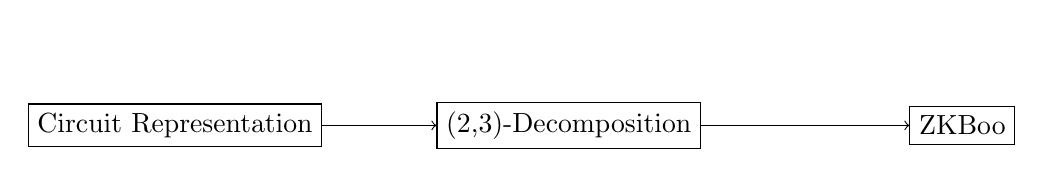
\begin{tikzpicture}
      \node[draw] at (-20,.3) (a) {Circuit Representation};
      \node[draw] at (-15,.3) (b) {(2,3)-Decomposition};
      \node[draw] at (-10,.3) (c) {ZKBoo};

      % draw edges
      \draw[->] (a) -- node[midway,above,yshift=1cm] {} (b);
      \draw[->] (b) -- node[midway,above] {} (c);
  \end{tikzpicture}
  \caption{\label{fig:outline_zkboo} Outline of ZKBoo formalisation}
\end{figure}

\paragraph{Preliminary notation}
Throughout this chapter use the letter $e$ to denote an integer in \{1,2,3\}.
Moreover, we define arithmetic on $e$ such that $3+1 = 1$.

\section{Formalising Arithmetic circuits}
\label{sec:arith_circuits}
In this section we will introduce the concept of arithmetic circuits and how they
can be represented. Primarily we recall the usual definition of circuits as
graph and discuss how to evaluate circuits programmatically. From this we
introduce a number of restrictions to our formalisation which makes their easier
to work with, whilst still being expressive enough to use in the ZKBoo protocol.
Based on these restrictions we then formulate an alternative representation for
arithmetic circuits and give a number of key definitions, which are needed for
reasoning about the structure of a circuit and the evaluation of circuits.

\subsection{Representing an arithmetic circuit}
\label{subsec:arith-representation}
An arithmetic circuit is in its most general form express a function $\phi$ over some
arbitrary field $\mathbb{Z}_{q}$, where $\phi : \mathbb{Z}_{q}^{k} \rightarrow \mathbb{Z}_{q}^{l}$

To express arbitrary (Arithmetic) computations in a ring of finite field we
use the following four gates, Add to constant (ADDC), multiply by constant
(MULTC), addition of two wires (ADD), and multiplication of two wires (MULT).

The goal of this section is to formulate a representation of the function
$\phi$, which only depends on the aforementioned gate types to perform
computations. Before doing so, however, we start by stating a number of
simplifying assumptions about our arithmetic circuits. First, we only allow the
circuit to have one input value and one output value, in other words:
$k = l = 1$ in the definition of $\phi$.
This assumption exists pure to make it easier to reason about the inputs and
output of the function. The formalisation in this section could be altered to
allow for arbitrary inputs with minor alterations, which we will discuss later.
\todo{Discuss this later}

Based on these simplifying assumptions we can now recall the graph
representation of a circuit:
\begin{definition}[Arithmetic Circuit]
  \label{def:arith_circuit}
  An Arithmetic circuit is a graph C = (W, G) where W is the internal
  wires between the gates and G is the set of gates within the circuit. Then,
  we let $i \in G$ be first gate of the circuit, i.e. its only input and $o \in G$ be the output
  gate, for which there must exists a path from i to o in W.
  Specifically, o is a gate with only one in-going wire and no out-going wire.
  The means that the value of the circuit can be read by reading the value of
  the in-going wire to o.

  \todo{Define in- and out-wires?}

  Finally, for all gates $g \in G$ there must exists path in W from i to o going
  through g,
  since if this was not the case, the gate does not contribute the output of the
  gates and can therefore be removed from the graph without changing the
  semantic meaning of the circuit.
\end{definition}

To define evaluation of a circuit we would then need compute the value of the
in-wire of o, but this can only be done if we have computed all other wires in
the circuit. Moreover, the value of the out-wires of a given gate, g, can only
be computed if all in-wires of g has already been computed to a value. It is
clear from this that we need to define an order of evaluation, such that we only
try to compute the out-wire of a gate if we know that all in-wires has been computed.

To define the order of evaluation we follow the work of \cite{Yao} and introducing an alternative
representation of Arithmetic circuits, which naturally gives us a well-defined
evaluation order:

\begin{definition}[List representation of arithmetic circuits]
  Given an arithmetic circuit C as defined by definition \ref{def:arith_circuit}
  we define the list representation of C as computing a linear ordering, O, of
  G, which gives each gate in G an unique index.
  \todo{Why do we remove i and o?}
  We then let the list representation $C_{L}$ be defined as:
  \[
    C_{L}[j] = Enc(O( G \setminus \{i\})[j], W)
  \]

  Where $Enc : gate \rightarrow W \rightarrow \text{encoded gate}$, is a function
  taking as input a gate and the wires of the circuit and produces an encoded
  gate.
  The encoded gate contains type information about gate but also stores the
  indexes (From the linear ordering) of the gates, whose out-going wires are the
  in-going wires of the gate.
  The type declaration of the encoded gates can be seen in figure \ref{lst:gate_types}.
\end{definition}

\todo{Tikz example showing the two representations}

\todo{This representation does not allows for optimisations like parallel computations}

\paragraph{Linear ordering}
A linear ordering O is a function that when applied to G assigns a unique
index to each gate in G.
One example of such function defining a linear ordering is a breadth-first
search, where each gate in the circuit graph is labelled according to at which
time the BFS reached the gate.
This labelling would start at gate $i$ and end at $o$.

A special property of the linear ordering induced by a BFS labelling is that a
gate can only be visited when all nodes that the gates computation can depend on
has already been visited. This ensure that for a node indexed $i$ it only
depends on out-wires of nodes with index less-than $i$.

This ordering allows us to convert the graph representation into a list
representation, where the gate at index $i$ is the node with index $i$ by the
linear ordering. However, since the gates $i$ performs no computation and only
exists to add the input value to the graph we exclude it from the list
representation, and shift every index one down.

\paragraph{Encoded gates}
A gate is then a type, which defined its operation along
with a tuple $(l,r)$ where $l$ is the index of left input wire and $r$ is the
index of the right input wire. In the case of unary gates like ADDC and MULTC
the tuple is $(l, c)$ where l is the input wire and $c$ is the constant used in
the computation.

But we need to encode W into this list. To do this we encode the information
about input wires into the types of the gates themselves, as seen in figure
\ref{lst:gate_types}.

\begin{lstlisting}[float,label=lst:gate_types,caption=Type declaration of gates]
type encoded_gate = [
  | ADDC of (int * int)
  | MULTC of (int * int)
  | MULT of (int * int)
  | ADD of (int * int)
].
\end{lstlisting}
\vspace{2mm}
\noindent
One important aspect of the list representation of circuits is that it allows
us to easily define an evaluation order, where we are ensure that we are not
computing the value of a gate before the previous gates has been computed. To
capture this notion of a valid evaluation order we give the following definition:

\todo{Define notation for list indexing?}

\begin{definition}[Valid circuit]
  \label{def:decomp:valid_circuit}
  An arithmetic circuit in list representation $C_{L}$ is valid if for every
  entry $i$ in the list it holds that:
    \begin{itemize}
      \item C[i] is a gate type
      \item the input wires of C[i] have index less than $i$.
      \item the input wires of C[i] have index greater than or equals to $0$.
    \end{itemize}
\end{definition}

\begin{lstlisting}[float,label=lst:circuit_eval,caption=Circuit evaluation function]
op eval_gate (g : gate, s : int list) : int =
  with g = MULT inputs => let (i, j) = inputs in
                          let x = (nth 0 s i) in
                          let y = (nth 0 s j) in x * y
  with g = ADD inputs =>  let (i, j) = inputs in
                          let x = (nth 0 s i) in
                          let y = (nth 0 s j) in x + y
  with g = ADDC inputs => let (i, c) = inputs in
                          let x = (nth 0 s i) in x + c
  with g = MULTC inputs => let (i, c) = inputs in
                          let x = (nth 0 s i) in x * c.

op eval_circuit_aux(c : circuit, s : int list) : int list =
    with c = [] => s
    with c = g :: gs =>
     let r = eval_gate g s in
     eval_circuit_aux gs (rcons s r).

op eval_circuit (c : circuit, s : state) : output =
    last 0 (eval_circuit_aux c s).
\end{lstlisting}

From this representation of circuits as a list of gates, where gates are types,
it is possible to define the semantic meaning of this representation, by
defining the evaluation function, which can be seen in figure \ref{lst:circuit_eval}.
The evaluation is broken into two parts: First we have a function for evaluating
one gate to an intermediate values. Second, we have a procedure for evaluating
the entire circuits which calls the former function.
To evaluate a single gate, we first need to determine which gate it is. This can
be done by utilizing the power of the \easycrypt\ type system, which allows us
to pattern match on the type of the gate as seen in listing \ref{lst:circuit_eval}.

Then, if the circuit is valid the evaluation order is the indexes of the list representation.
We know that if we are computing index $i$ of the circuit, then indices
$[0 \dots i-1]$ have already been computed. Perform the appropriate function
then reduces to looking up the values of the previously computed gates and
applying them to the function appropriate for the type of the gate.

Computing the entire circuit then follows from the same fact, that gates are always
evaluated in the order the appear in the list, and the no gate can depend on
the result of gates, which have a higher index than itself. By continually
performing gate evaluation of the next entry in the list and saving the result
into ``state'' where each index correspond to the computed value of the gate at
that index in the circuit, and the calling recursively on the list with the
first entry removed, then the output of the gate will be in the last entry of
the state, when there are no more gates to compute. Assuming that there is only
one output gate.

\begin{definition}[State of list representation]
  For a list representation of a circuit $C_{L}$ we give the following recursive
  definition of the state:
  \begin{align*}
    \text{state}[0] &= \text{input value} \\
    \text{state}[i>0] &= \texttt{eval\_{gate} } C_{L}[i-1] \; state[i-1]
  \end{align*}

  Here we recall that input gate has been removed from the list representation
  and $C_{L}$[0] is the first non-input gate in the circuit. From this it also
  follows that
  \begin{equation}
    \text{size } \text{state} = \text{size } C_{L} + 1
  \end{equation}
\end{definition}

We then have that any valid circuit c can be compute to a value y as
\texttt{eval\_circuit(c, [input]) = y}. This can also be stated as a probabilistic
procedure as $\Pr{\texttt{eval\_circuit(c, [input])} = y} = 1$.

To reason about functions and procedures about functions we have the following lemma:
\begin{lemma}[Function/Procedure relation]
  \label{lem:func/proc-equiv}
  $\forall$ f, inputs, output: f(inputs) = output $\iff \Pr{f(inputs) = output} = 1$.
\end{lemma}
\begin{proof}
  \hspace{2mm}
  \begin{itemize}
    \item  ``$\Rightarrow$'':
      Trivial
    \item  ``$\Leftarrow$'':
      by contradiction?
  \end{itemize}
\end{proof}

\todo{ZKBoo paper gives no notion of a valid evaluation order - needed for security}

\todo{Graph representation isomorphic to list representation?}


\section{(2,3) Decomposition of circuits}
\label{sec:decomposition}
In this section we ... formalisation based on the description of arithmetic circuits...
\todo{mention MPC}

In its most general form, we can define the decomposition as a procedure taking
as input three views and random tapes, and a circuit and produces three new
views. \todo{rewrite? - Random tapes = set of random choices}
More specifically the decomposition work by incrementally evaluating a gate based on
previously compute views, which yield new shares that can be appended to the
view. This process of evaluating a single gate based on the view of evaluating
the previous gate can then be repeated until all gates have been computed. This
overall idea has been captured in the procedure in figure \ref{lst:decomp_aux},
where it is assumed access to a function eval\_gate, which has signature:
$eval\_gate : circuit \Rightarrow party \Rightarrow (view * view) \Rightarrow (random\_tape * random\_tape) \Rightarrow share$,
\todo{explain eval gate better?}
where $party$ is a integer in $\{1,2,3\}$ that determines which party is
computing the share. \todo{Say that eval gate implements the function in the
  ZKBoo section}

The output of the decomposition can then be defined as summing the last share from each view that has been compute by the aformentioned procedure. More formally the output is:
\begin{equation}
  \text{Output}(w1, w2, w3) = \sum_{i \in \{1,2,3\}} \text{last } w_{i}
\end{equation}


\begin{definition}[Correctness of views]
  \label{def:decomp:valid_view}
  For any three views (list of shares), $w_{1}, w_{2}, w_{3}$, with equal length, we
  say that they contain valid shares of computing a circuit c, if it holds:

  \begin{equation}
    \label{eq:decomp:view:sum}
    \forall 0 \leq i < \text{size } c,
      \sum_{p \in \{1,2,3\}} w_{p}[i] = s[i]
  \end{equation}

  where s is the list of intermediate values produces by calling
  \texttt{eval\_circuit\_aux} in figure \ref{lst:circuit_eval}.

  Additionally a share is only valid, if it has been produced by functions used
  by the decomposition.

  \begin{equation}
    \label{eq:decomp:valid}
      \forall 0 \leq i < \text{size
                                                   } c - 1,  w_{e}[i+1] = \texttt{eval\_gate } c[i]\; w_{e} \; w_{e+1}
  \end{equation}

  To express that the views satisfy the above definition we use the notation
  \validviews{c,w1,w2,w3} to express that $w1, w2, w3$ are valid views for the
  decomposition of $c$

\end{definition}


\begin{lstlisting}[float,label=lst:decomp_aux,caption= Incremental decomposition procedure]
  proc compute(c : circuit, w1 w2 w3 : view, k1 k2 k3 : random_tape) = {
    while (c <> []) {
      g = oget (ohead c);
      r1 <$ dinput;
      r2 <$ dinput;
      r3 <$ dinput;
      k1 = (rcons k1 r1);
      k2 = (rcons k2 r2);
      k3 = (rcons k3 r3);
      v1 = eval_gate g 1 w1 w2 k1 k2;
      v2 = eval_gate g 2 w2 w3 k2 k3;
      v3 = eval_gate g 3 w3 w1 k3 k1;
      w1 = (rcons w1 v1);
      w2 = (rcons w2 v2);
      w3 = (rcons w3 v3);
      c = behead c;
    }
    return (k1, k2, k3, w1, w2, w3);
  }
\end{lstlisting}

\paragraph{Handing randomness}
\label{subsec:decomp:randomness}
Looking at compute we see that compute we make three random choices for each gate and then save those choices to some random tapes. These tapes are then returned. They are used to keep track of the random choices made thoughout the protocol, such that views can be verified. For most proof the specific values contained within the random tapes are not imporant, since the random values are only there to cancel eachother out whilst making the shares look randomly distributed.
We therefore omit the random tapes for most procedures and proofs in this section, since they are static?
When the random tapes are imporant for the security we will mentioned how.

The reason for sampling random values at each iteration of the while loop instead of all at once is to be able to reason about the specific random choices made at this time in the computation. This is especially important to be able to relate two procedures running at the same iteration of the while loop...


\subsection{Correctness}
\label{sec:decomp_correct}
Ultimately want to prove:
\begin{lemma}[Decomposition correctness]
  \label{lem:decomposition_correctness}

  \[
    \Pr{\texttt{eval\_circuit(c, [input])} = y} =
    \Pr{\texttt{decomposition(c, [input])} = y}
  \]

  i.e. The output distribution of the two programs are perfectly indistinguishable. From lemma \ref{lem:func/proc-equiv} we have that circuit evaluation always succeeds. This lemma, therefore, also implies that the decomposition always succeeds.
\end{lemma}

To prove the above lemma we first introduce a helper lemma:

\begin{lemma}[Stepping lemma for decomposition]
  \label{lem:decompose_compute_step}
  For any valid circuit c in list representation, it is possible to split the circuit into two parts
  $c_{1}, c_{2}$ where $c = c_{1} ++ c_{2}$ (++ is list concatenation).
  let $w_{1}, w_{2}, w_{3}$ be the resulting views of decomposing $c$ and
  \validviews{c_{1}, w_{1}, w_{2}, w_{3}} and let computing $c_{2}$ with initial
  views $w_{1}, w_{2}, w_{3}$ output views $w'_{1}, w'_{2}, w'_{3}$.
  Then \validviews{c, w'_{1}, w'_{2}, w'_{3}}.

  Alternatively this is stated as:
  \[
    \textbf{Valid}(c_{1}, w_{1}, w_{2}, w_{3})  \implies
    \Pr{ \texttt{compute}(c_{2}, w_{1}, w_{2}, w_{3}) : \textbf{Valid}(c, w'_{1} , w'_{2}, w'_{3}) } = 1
  \]

\end{lemma}
\begin{proof}
  The proof proceeded by induction on the list c.

  \begin{itemize}
    \item Base case $c = []$:
        trivially true since an empty circuit is the identity function.
    \item Induction step $c = c' ++ [g]$:
      \begin{itemize}
        \item Inline definitions to get compute\_stepped
        \item We use to induction hypotheses to compute c' which give us
              \validviews{c_{1}, w_{1}, w_{2}, w_{3}}.
        \item We then need to prove, that we can compute any gate on top of the
          valid views to produce a new set of valid views.
      \end{itemize}
  \end{itemize}

\end{proof}

\begin{proof}[Proof of lemma \ref{lem:decomposition_correctness}]
  By unfolding the definition we are left with proving that the last share from
  each of the views produced by \texttt{compute} are equal to the output of
  evaluating the circuit, which is true by lemma \ref{lem:decompose_compute_step}
\end{proof}

\todo{Our formalisation differs by imposing stricter restrictions on the shares computed...}


\subsection{2-Privacy}
\label{sec:decomp_privacy}
To prove 2-Privacy we need to first define a simulator capable of producing
indistinguishable views for two of the parties. To simulator is given by the
procedure \texttt{simulate} and function \texttt{simulator\_eval} in figure \ref{lst:zkboo:simulator}.
\texttt{simulator\_eval} is a function that evaluates a single gate from the
point of view of party ``p''. In the cases of evaluating ADDC ADD MULTC gates
the simulator simply calls the \texttt{eval\_gate} function, since these
computations are performed ``locally'' for each party, i.e. they do not depend
on the shares from the other parties in the protocol.
When evaluating MULT gates shares needs to be distributed amongst the parties,
but to evaluate the output of the MULT gate for any given party it only depends
on the parties own share and the share of the ``next'' party, i.e. for party one
he only depends on his own shares and the shares from party two. Since
the simulator simulates the view of party $e$ and $e+1$ the view of party $e$
can be computed normally with the \texttt{eval\_gate} function. For simulating
the view of party $e+1$ we use the fact that shares should be uniformly random
distributed, and simply sample a random value for the view.
This is true by equation \todo{Make sim mult function in zkboo chapter}, where
the difference between two random values are added to the share, effectively
making the share appear random too.
\todo{rewrite this}
In this case the view of party $e$ can always be computationally reconstructed
by looking at the view of party $e+1$, but the view of party $e+1$ cannot be
verified, since the view of party $e+2$ is unknown, which makes it seem valid.

\todo{Where we use that compute and simulate sample randomness at the time of computation}

The procedure $\texttt{simulate}$ is simply a wrapper around
\texttt{simulator\_eval}, which is responsible for constructing the views and
sampling randomness incrementally for each gate in the circuit, much like how \texttt{compute} is a wrapper around \texttt{eval\_gate}.

\begin{lstlisting}[float,label=lst:zkboo:simulator,caption= Simulator]
op simulator_eval (g : gate, p : int, e : int, w1 w2 : view, k1 k2 k3: int list) =
with g = MULT inputs =>
  if (p - e %% 3 = 1) then (nth 0 k3 (size w1 - 1)) else eval\_gate g p w1 w2 k1 k2
with g = ADDC inputs =>
    eval\_gate g p w1 w2 k1 k2
with g = MULTC inputs => eval\_gate g p w1 w2 k1 k2
with g = ADD inputs => eval\_gate g p w1 w2 k1 k2.

proc simulate(c : circuit, e : int, w1 w2 : view, k1 k2 k3 : random_tape) = {
  while (c <> []) {
    g = oget (ohead c);
    r1 <$ dinput;
    r2 <$ dinput;
    r3 <$ dinput;
    k1 = (rcons k1 r1);
    k2 = (rcons k2 r2);
    k3 = (rcons k3 r3);
    v1 = simulator_eval g e e w1 w2 k1 k2 k3;
    v2 = simulator_eval g (e+1) e w2 w1 k1 k2 k3;
    w1 = (rcons w1 v1);
    w2 = (rcons w2 v2);
    c = behead c;
  }
\end{lstlisting}

To compare the views output by the simulator and the ones produced by the decomposition we fix two procedures \texttt{real} and \texttt{simulated}, where the first return two views and the final share of the third view and the latter returns the two views output by the simulator and a fake final share of the thrid view. These procedures can be seen in figure \ref{lst:decomp-real-ideal}.

\begin{lstlisting}[float, mathescape,label=lst:decomp-real-ideal,caption= Real/Simulated view of decomposition]

proc real((c,y) : statement, w : witness, e : challenge) = {
    $(y_{1},y_{2},y_{3},w_{1},w_{2},w_{3})$ = compute(c);
    return $(w_{e}, w_{e+1}, y_{e+2})$
}

proc simulated((c, y) : statement, e : challenge) = {
    $(w_{e}, w_{e+1})$ = simulate(c, e);
    $y_{e}$ = last $w_{e}$;
    $y_{e+1}$ = last $w_{e+1}$;
    $y_{e+2}$ = $y - (y_{e} + y_{e+1})$
    return $(w_{e}, w_{e+1}, y_{e+3})$
}

\end{lstlisting}

We are then ready to state 2-privacy as the following lemma:
\begin{lemma}[Decomposition 2-Privacy]
  \label{lem:zkboo:decomposition:privacy}
  We say that the decomposition protocol offers 2-Privacy, if the output
  distributions between \texttt{real} and \texttt{simulated} are
  indistinguishable.

  \todo{Why must h be in the domain of R here, but not in correctness?}

  This can be stated in rPHL as:
  \[
    h \in \textbf{Domain}(R) \implies
    equiv[real \sim simulated : =\{e, h\} \implies =\{res\}].
  \]

\end{lemma}

To prove this lemma we first prove that running \texttt{compute} and
\texttt{simulate} with the same random choices will produce indistinguishable
views corresponding to the challenge and summing the output shares of
\texttt{compute} will yield the same value as evaluating the circuit. This
effectively inlines the correctness property in the proof of the simulator. This
is necessary to be able to reason about the existence of the view of party
$e+2$, which would make the views produced by the simulated equal to honestly
produces views.
More specifically the inlined correctness property gives us ...

This is stated as the following lemma:

\todo{Define notation for referring the views from protocol one and the views
  from protocol 2}

\begin{lemma}
  \label{lem:zkboo:decomposition:privacy_aux}
  Given a valid arithmetic circuit in list representation with challenge $e$ and
  intermediate circuit computations/state $s$ the following holds:

  \[
    equiv[compute \sim simulated : \; =\!\{h, e, w_{e}, w_{e+1}\} \implies =\!\{w'_{e}, w'_{e+1}\}]
  \]

  Moreover, we require that the input views $w_{1}, w_{2}, w_{3}$ satisfies the
  correctness property from equation \ref{eq:decomp:view:sum}.

  Additionally this property most also hold for the views
  $w'_{1}, w'_{2}, w'_{3}$ produced by running \texttt{compute}. This is
  equivalent to part of the \textbf{Valid} property used in the proof of
  correctness.

  % \begin{itemize}
  %   \item Running \texttt{compute} and \texttt{simulate} with the same random
  %     choices satisfies conditions:
  %     \begin{itemize}
  %       \item The initial views of $w^{compute}_{e}$ and $w^{compute}_{e+1}$ are indistinguishable from  $w^{simulate}_{e}$ and $w^{simulate}_{e+1}$.
  %       \item It hold that $\forall 0 \leq i < size w1, w_{1}[i] + w_{2}[i] + w_{3}[i] = s[i]$
  %       \item
  %     \end{itemize}
  % \end{itemize}
\end{lemma}
\begin{proof}
  We proceed by induction on the list representation of the circuit c:

  \begin{itemize}
    \item Base Case $c = []$ : trivial
    \item Induction Case $c = g::cs$ :
    \item Write this as program steps like in \cite{certicrypt_sigma}?
      \begin{align*}
        compute(g::gs, w_{1}, w_{2}, w_{3}) \sim simulate(g::gs, w'_{1}, w'_{2}, w'_{3} )
      \end{align*}
  \end{itemize}

\end{proof}

\begin{proof}[Proof of lemma \ref{lem:zkboo:decomposition:privacy}]
  By applying lemma \ref{lem:zkboo:decomposition:privacy_aux} we have that the
  views output by both procedures are indistinguishable. All we have left to prove
  is that $y^{real}_{e+2} \equiv y^{simulated}_{e+2}$. To prove this we use the
  equation \ref{eq:decomp:view:sum}, which states that the shares of the real views always sum to
  the intermediate values of computing the circuit to conlude
  \[
  y = y^{real}_{1} + y^{real}_{2} + y^{real}_{3} \iff y^{real}_{e+2} = y - (y^{real}_{e} + y^{real}_{e+1})
  \]
  Then by
  $(y^{real}_{e} + y^{real}_{e+1}) \equiv (y^{real}_{e} + y^{real}_{e+1})$ it
  follows that
  \begin{align*}
    y^{real}_{e+2} &= y - (y^{real}_{e} + y^{real}_{e+1}) \\
                      &\equiv y - (y^{simulated}_{e} + y^{simulated}_{e+1}) \\
                      &= y^{simulated}_{e+2}
  \end{align*}
\end{proof}


\section{ZKBOO}
\label{sec:formal_zkboo}
\todo{Throughout this section we will introduce the instantiated sigma protocol...}
Since the ZKBoo protocol is an instantiation of a $\Sigma$-Protocol we start by
defining the types as specified in section \ref{ch:formal_sigma}.

\lstinputlisting[linerange={13-17}]{../code/ZKBoo.ec}

% and instantiating the $\Sigma$-Protocol framework.

The relation is then all tuples of circuits outputs and inputs, where it holds that evaluating the circuit with the input returns the output. We formally encode this as
\begin{equation}
  \text{R } = \{((c,y), w) \,|\, \texttt{eval\_circuit } c \; w = y\}.
\end{equation}

We then add the restriction, that the challenge is always a integer in
$\{1,2,3\}$. Moreover, we recall from section \ref{sec:zkboo}, that ZKBoo
depends on a commitment scheme. Here we follow \cite{zkboo} and use a key-less
commitment scheme. We therefore assume the existence of a commitment scheme,
Com, which is an instantiation of the key-less commitment scheme formalisation
from section \ref{sec:formal_zkboo}. Furthermore, we simply our proof burden by
requiring Com to satisfy the alternative perfect hiding property from definition
\ref{def:commitment:perfect-hiding} as well as the alternative binding property
from definition \ref{def:commitment:alt-binding} with probability $binding\_prob$.

With these preliminaries in place we are now ready formalise the ZKBoo protocol.
First, we start by defining the sub-procedures needed for the \texttt{verify}
procedure. Recall from section \ref{sec:zkboo}, that the Verifier accepts a
transcript $(a,e,z)$ if $z$ is a valid opening of the views $w_{e}$ and
$w_{e+1}$ commitment to in $a$ and that every entry in $w_{e}$ has been produced
by the procedure defining the decomposition. This step of validating that
$w_{e}$ has been produced in accordance with the decomposition is given 
by equation \ref{eq:decomp:valid}.
%
This equation can be encoded within \easycrypt\ as a predicate:
\todo{Change the procedure to use the naming from the report}
\lstinputlisting[linerange={47-50}]{../code/ZKBoo.ec}

Predicates allows us to use quantifiers to assert properties within \easycrypt , which are nice to
reason about especially in pre and post condition of procedures. Predicates,
however, have no computation aspect to them and are pure logical.
Having a predicate reasoning quantifying over all integers, for example, is
perfectly legal, but this is obviously not possible to express as a computation,
since it would take indefinitely many computations to verify a property for
indefinitely many integers.
A predicate, therefore, cannot be used within procedures, since they are not
required to be computable.
The quantification in equation \ref{eq:decomp:valid}, however, only need
finitely many computations to verify the property, since it is bounded by the
size of the circuit. We can, therefore, define a computable function which for
each entry check if the property holds and then returns if the property holds
for all entries. This can clearly be computed in time proportional to the size
of the circuit and the time it takes to compute one share of the decomposition.
This function is given by:
\lstinputlisting[linerange={51-54}]{../code/ZKBoo.ec}

This function allows us to computationally validate the property from equation
\ref{eq:decomp:valid}, but it is harder to reason about, since we have
to reason about every computational step of the function before we can verify
the property holds. We would therefore want our function to use our function in
the implementation of ZKBoo, but use the predicate whenever we need to reason
about the security of the protocol. To achieve this we introduce the following
lemma, which allows us to use the predicate over the function when applicable:
\begin{lemma}[valid\_view predicate/op equivalence]
  $\forall$ p, w1, w2, c, k1, k2:
  valid\_view p w1 w2 c k1 k2 $\iff$ valid\_view\_op p w1 w2 c k1 k2
\end{lemma}

With a way to validate the views we can instantiate the ZKBoo protocol from
section \ref{sec:zkboo} as a $\Sigma$-Protocol in our formalisation by
implementing the algorithms from figure \ref{lst:sigma_procedures}, which can be
seen in figure \ref{lst:zkboo_procedures}.
\todo{Assumes existence of decomposition protocol}

\begin{lstlisting}[float, mathescape,label=lst:zkboo_procedures,caption= ZKBoo $\Sigma$-Protocol instantiation]
global variables = w1, w2, w3, k1, k2, k3.

proc init(h : statement, w : witness) = {
  (x1, x2, x3) = Share(w);
  (k1, k2, k3, w1, w2, w3) = Decompose(c, x1, x2, x3);
  $c_i$ = Commit($(w_{i}, k_i)$);
  $y_{i} = $ last 0 $w_{i}$;
  return (y1, y2, y3, w1, w2, w3);
}

proc response(h : statement, w : witness, m : message, e : challenge) = {
  return $(k_e, w_{e}, k_{e+1}, w_{e+1})$
}

proc verify(h : statement, m : message, e : challenge, z : response) = {
  (y1, y2, y3, c1, c2, c3) = m;
  (c, y) = h;

  (k1', w1', k2', w2') = open;
  valid_com1 = verify $(w'_{e}, k'_{e})$ c1;
  valid_com2 = verify $(w'_{e+1}, k'_{e+1})$ c2;
  valid_share1 = last 0 $w'_{e}$ = y1;
  valid_share2 = last 0 $w'_{e}$ = y2;
  valid = valid_view_op 1 $w'_{1}$ $w'_2$ c $k'_1$ $k'_2$;
  valid_length = size c = size $w'_e - 1$ /\ size $w'_{1}$ = size $w'_2$;

  return y = y1 + y2 + y3 /\ valid_com1 /\ valid_com2 /\ valid_share1 /\ valid_share2 /\ valid /\ valid_length
}

\end{lstlisting}

We then, automatically, by our formalisation of $\Sigma$-Protocols get
definition of security and only need to prove them \dots \todo{wording}

\begin{lemma}
  \label{lem:zkboo:correctness}
  ZKBoo satisfy $\Sigma$-Protocol completeness definition \ref{def:sigma:completeness}.
\end{lemma}
\begin{proof}
We start by observing that committing to $(w_{i}, k_{i})$ in \texttt{init} and
the verifying the commitment in \texttt{verify} is equivalent to the correctness
game for commitment schemes defined in \ref{ch:formal_commitment}.

We therefore inline the completeness game, and replace the calls to the
commitment procedures with the correctness game:

\begin{lstlisting}[mathescape, label=lst:zkboo-inter-completeness,caption=
Intermediate game for completeness]
proc intermediate_main(h : statement, w : witness, e : challenge) = {
  (c, y) = h;
  (x1, x2, x3) = Phi.share(w);
  (k1, k2, k3, w1, w2, w3) = Phi.compute(c, [x1], [x2], [x3]);
  $y_{i}$ = last 0 $w_{i}$;

  valid_com1 = Correctness.main($(w_e, k_e)$);
  valid_com2 = Correctness.main($(w_{e+1}, k_{e+1})$);
  commit($(w_{e+2}, k_{e+2})$);
  valid_share1 = valid_view_output $y_{e}$ $w_{e}$;
  valid_share2 = valid_view_output $y_{e+1}$ $w_{w+1}$;
  valid = valid_view_op e $w_{e}$ $w_{e+1}$ c $k_{e}$ $k_{e+1}$;

  valid_length = size c = size $w_{e} - 1$ /\ size $w_{e}$ = size $w_{e+1}$;

  return valid_output_shares y y1 y2 y3 /\ valid_com1 /\ valid_com2 /\ valid_share1 /\ valid_share2 /\ valid /\ valid_length;
}
\end{lstlisting}

We then prove the correctness of \texttt{intermediate\_main} by showing that
the procedure returns true for any $e \in \{1,2,3\}$.

\vspace{3mm}
\noindent
\textbf{Case} $e = 1$:
For the procedure to return true we need to following to hold:

\begin{itemize}
  \item All variables must be true
  \item commit must be lossless such that procedure always terminates
    \begin{itemize}
      \item commit must be lossless by completeness of commitment scheme
      \item formalise this?
    \end{itemize}
\end{itemize}

The other cases are the same.

\end{proof}

\begin{lemma}
  Assuming perfect hiding from definition \ref{def:commitment:perfect-hiding} then ZKBoo satisfy Special Honest Verifier Zero-knowledge definition \ref{def:sigma:shvzk}
\end{lemma}
\begin{proof}
  To prove shvzk we show that running the \texttt{real} and the \texttt{ideal}
  procedures with the same inputs and identical random choices produces
  indistinguishable output values. The proof the proceeded by casing on the
  value of the challenge $e$. To proof for the different values are identical so
  we suffice in showing only the case of $e=1$. When $e=1$ the two procedures
  are:

  \begin{figure}[ht]
    \centering
    \begin{subfigure}{0.48\textwidth }
    \begin{lstlisting}[mathescape]
proc real(h, w, e) = {
  (x1, x2, x3) = Share(w);
  (k1, k2, k3, w1, w2, w3) = compute(c, x1, x2, x3);
  $c_i$ = Commit($(w_{i}, k_i)$);
  $y_{i} = $ last 0 $w_{i}$;

  a = $(y_{1}, y_{2}, y_{3}, c_{1}, c_{2}, c_{3})$
  z = $(k_e, w_{e}, k_{e+1}, w_{e+1})$

  if (verify(h,a,e,z)) {
    Some return (a,e,z);
  }
  return None;
}
    \end{lstlisting}
    \end{subfigure}
    \hfill
    \begin{subfigure}{ 0.48\textwidth }
    \begin{lstlisting}[mathescape]
proc ideal(h, e) = {
    (* From Decomposition *)
    $(w_{e}, w_{e+1}, y_{e+2})$ = simulated;

    (* Generate random list of shares *)
    $w_{e+2}$ = dlist dinput (size $w_{1}$);
    $k_{e+2}$ = dlist dinput (size $k_{1}$);
    $y_{e}$ = last 0 $w_{e}$;
    $y_{e+1}$ = last 0 $w_{e+1}$;
    $c_{i}$ = commit($(w_{i}, k_{i})$);
    a = $(y_{1}, y_{2}, y_{3}, c_{1}, c_{2}, c_{3})$;
    z = $(w_{e}, w_{e+1})$;

    if (verify(h,a,e,z)) {
      Some return (a,e,z);
    }
    return None;
}
    \end{lstlisting}
    \end{subfigure}
  \end{figure}

  By 2-Privacy of the decomposition we know that \texttt{compute} and
  \texttt{simulate} are indistinguishable procedures, when the view $e_{e+2}$
  produced by \texttt{compute} is never observed. This is fortunately the case
  here, we when calling the sub-procedure \texttt{simulate} in the ideal case,
  we know that the properties ensured by the correctness of the decomposition
  must also hold in the ideal case. This means that the views produced by
  \texttt{simulate} must also produce views which satisfy the correctness
  property for the views \ref{def:decomp:valid_view}.
  This is enough to make the \texttt{verify} procedure return true.

  We, therefore, only need to argue that $c_{e+2}$ are identically distributed
  for both of the procedures. In the real case $c_{e+2}$ is simply committing to
  the view produces by the decomposition. In the ideal case, however, it is a
  commitment to a list of random values but due out assumption of perfect hiding
  these two commitments are identically distributed.

  The rest of the out values are indistinguishable by the 2-Privacy property.

\end{proof}

\todo{Change order so this lemma comes last}
\todo{Problem: compute sample random values - tape is complete already in this instance}
\begin{lemma}
  Given a commitment scheme, where an adversary can produce three pairs
  commitments, where at least one pair has different openings with probability
  $p$, then ZKBoo satisfy the 3-Special Soundness property with probability $p$.
\end{lemma}
\begin{proof}
  The proof has three distinct steps.
  First, we show that the inputs z1, z2, z3 to \texttt{witness\_extractor}
  procedure will be valid and consistent openings revealing the views
  $w_{1}, w_{2}, w_{3}$ which has been produced by the same call to \texttt{compute}
  with probability $1-p$. Next, we show that given views $w_{1}, w_{2}, w_{3}$
  which correspond to three views produced by the same call to \texttt{compute},
  then a valid witness can be extracted.
  Ultimately, we show that Special Soundness game can be won with probability $(1-p)$

  \paragraph{Consistent views}
  To check if the views are valid we use the \texttt{verify} procure, which
  check that \texttt{valid\_view\_op} return true. By lemma
  \ref{lem:func/proc-equiv} we know that this is equivalent to equation
  \ref{eq:decomp:valid}. From this we can define the following procedure for
  checking validity and consistency of the openings:

\begin{lstlisting}[label=lst:zkboo:consistency,caption=Consistency procedure]
proc extract_views(h : statement, m : message, z1 z2 z3 : response) = {

  v1 = verify(h, m, 1, z1);
  v2 = verify(h, m, 2, z2);
  v3 = verify(h, m, 3, z3);

  (w1, w2) = z1;
  (w2', w3) = z2;
  (w3', w1') = z3;
  (y1, y2, y3, c1, c2, c3) = m;
  cons = bind_three(c1, c2, c3, (w1, k1), (w1', k1'), (w2, k2), (w2', k2'), (w3, k3), (w3', k3'));

  return v1 /\ v2 /\ v3;
}
\end{lstlisting}

  Here we are given two potential openings for each view, namely $w_{e}$
  and $w'_{e}$. Ideally $w_{e} = w'_{e}$ but if it is possible for the adversary
  to win the binding game for three commitments then the openings might be
  inconsistent. We therefore let the procedure call \texttt{bind\_three}, which
  returns true if the adversary has broken the binding game. This is bound to a
  variable cons, which is not returned. This allows us to encode the consistency
  check as auxiliary information such that the return value of the procedure is
  still equivalent to only calling \texttt{verify} on the three responses.


  From this we can state the following:
  \begin{lemma}
    \label{lem:consistent-views}
    $\Pr{\texttt{extract\_views}(h, m, z_1, z_2, z_3) : v_1 \land v_2 \land v_3 \land w_{i} =
      w'_{i}} = (1-binding\_prob)$
  \end{lemma}
  \begin{proof}
    Special soundness assumes that all transcripts are accepting, we can
    therefore conclude that $v_{1} \land v_{2} \land v_{3}$ must hold.
    We are then left with showing that \texttt{bind\_three} proves that the
    views are consistent with probability $(1-binding\_prob)$. This is true by
    our assumption of Com having binding.
  \end{proof}

  % For any one of the openings only the view corresponding to the challenge needs
  % to be provably constructed by the decomposition. This means that we need all
  % three openings to conclude that the views has all been produced by the
  % decomposition. However, by breaking the binding property it is possible to
  % provide an opening, which might not have been produced by the same call to
  % \texttt{compute}. For example, z1 reveals $w^{1}_{1}, w^{1}_{2}$ whilst z2
  % reveals $w^{2}_{2}, w^{2}_{3}$, but if the binding property is broken, then
  % $w^{2}_{2}$ might be a valid view, but it has been produced with randomness
  % that is different from $w^{1}_{2}$. The probability of breaking the binding property is $p$,
  % hence the probability of all openings being to the same views is $1-p$.

  \paragraph{Witness extraction}
  Given that all openings correspond to the same call of \texttt{compute} and
  \validviews{c, w_1, w_2, w_3} we must then show that
  $w = w_{1}[0] + w_{2}[0] + w_{3}[0] \implies y = \texttt{eval\_circuit}(c, w)$
  i.e. the witness is the sum of all the input shares to the parties of the
  decomposition.

  \begin{align*}
    &\texttt{eval\_circuit}(c, w_{1}[0] + w_{2}[0] + w_{3}[0]) = y \\
    \iff& \Pr{\texttt{eval\_circuit}(c, w_{1}[0] + w_{2}[0] + w_{3}[0]) = y} \\
      =& \Pr{(w'_{1}, w'_{2}, w'_{3}) \leftarrow \texttt{compute}(c, w_{1}[0], w_{2}[0], w_{3}[0]); \left(\sum_{i \in \{1,2,3\}} \text{last
         }w'_{i} \right) = y}
  \end{align*}

  We then show that we can traverse the computations of the decomposition in
  reverse:
  \begin{lemma}
    \label{lem:witness-extraction}
      $\Pr{(w'_{1}, w'_{2}, w'_{3}) \leftarrow \texttt{compute}(c, w_{1}[0], w_{2}[0], w_{3}[0]); \left(\sum_{i \in \{1,2,3\}} \text{last }w'_{i} \right) = y}$
  \end{lemma}


  Now, we can it is possible to show that for each iteration of the while-loop
  in \texttt{compute} it must preserve the property that
  \[
    \forall j \in \{1,2,3\} \forall 0 \leq i < \text{size } w_{j}':\; w'_{j}[i] = w_{j}[i]
  \]
  by \validviews{c, w_1, w_2, w_3}, which asserts that each view has precisely
  been constructed by the \texttt{compute} procedure with the appropriate randomness.

  Moreover, we have that $\sum_{i \in \{1,2,3\}} \text{last }w_{i} = y$ since
  the transcripts containing the views are accepted by the \texttt{verify}
  procedure, which proves that the witness can be reconstructed if all the views
  of the decomposition is given.


  \paragraph{Special Soundness}
  The soundness game can be restated as the following procedure returning true
  with probability $1-p$
\begin{lstlisting}
proc alt_soundness(h, m, z1, z2, z3) = {
  v = consistent_views(h, m, z1, z2, z3);
  w = witness_extractor(h, m, [1;2;3], [z1;z2;z3]);

  if (w = None \/ !v) {
    return false;
  } else{
    w_get = oget w;
    return R h w_get;
  }
}
\end{lstlisting}
  \begin{lemma}
    \label{lem:soundness_alt_equiv}
    The above procedure has output distribution indistinguishable from the
    soundness game from definition \ref{def:sigma:soundness} instantiated with
    ZKBoo, i.e.
    $\Pr{\texttt{alt\_soundness}} = \Pr{\texttt{soundness(ZKBoo)}}$
  \end{lemma}
  \begin{proof}
    By inlining all sub-procedure calls from both procedures we have equivalent
    calls to \texttt{verify} and \texttt{witness\_extractor}. The only
    differences between the two procedures is that
    $\texttt{consistent\_{views}}$ call the binding game, but the value from the
    binding game is never returned, so it does it affect the output distribution.
  \end{proof}

  We can then show conclude the proof of the main lemma by
  applying lemma \ref{lem:soundness_alt_equiv}.
  From this we need to show:
  $\Pr{\texttt{alt\_soundness} : true} = (1- binding\_{prob})$.
  Which follows from applying lemma \ref{lem:consistent-views} and \ref{lem:witness-extraction}.
\end{proof}

\begin{lstlisting}[float,label=lst:zbkoo_extractor,caption= ZKBoo witness extractor]
proc witness_extractor(h : statement, a : message, e : challenge list, z : response list) = {
  [z1; z2; z3] = z;
  (k1'', w1'', k2'', w2'') = z1;
  (k2', w2', k3'', w3'') = z2;
  (k3', w3', k1', w1') = z3;

  if (k1'' = k1' /\ w1'' = w1' /\ k2'' = k2' /\ w2'' = w2' /\ k3'' = k3' /\ w3'' = w3') {
    ret = Some( (first 0 w1') + (first 0 w2') + (first 0 w3') );
  } else {
    ret = None;
  }
  return ret;
}
\end{lstlisting}


\todo{Formal verification does not tell us about efficiency}

\paragraph{Conclusion}
In this chapter we have seen how to apply our formalisations of
$\Sigma$-Protocols and commitment schemes to a MPC based protocol...

Formal proofs like these can help us gain insight into the security of the
protocols. The security of the ZKBoo protocol is entirely dependent on the
security properties of the underlying decomposition and commitment scheme being
state properly. For example, if the decomposition does not ensure that all the
shares in the views has been produced according to the decomposition algorithm,
then ZKBoo offers no guarantee about

Moreover, they help us expose some of the more subtle details important for
proving security of cryptographic protocols, like requiring certain procedures
to be lossless since...



%%% Local Variables:
%%% mode: latex
%%% TeX-master: "../main"
%%% End:


%%%%%%%%%%%%%%%%%%%%%%%%%%%%%%%%%%%%%%%%%%%%%%%%%%%%%%%%%%%%%%%%%%%%%%%

\chapter{Reflections and Conclusion}
\label{sec:reflection_conclusion}

\section{Related Work}
\label{sec:related_work}

This work exists in the field of formal verification of cryptographic protocols.
Notably our work has been heavily influenced by similar formalisations
\cite{cryptoeprint:2019:1185,DBLP:journals/corr/MetereD17,certicrypt_sigma,zkcrypt,Yao}

Sigma protocols has been done in a lesser extend in \easycrypt. Much of the same
work has been done in Isabelle/CryptHOL by \citeauthor{cryptoeprint:2019:1185}.

\citeauthor{certicrypt_sigma} formalised $\Sigma$-Protocols within CertiCrypt,
and proved the security of the $\Sigma^{\phi}$-Protocol, which proves knowledge
of the pre-image of a group homomorphism. ZKBoo protocol described in section
\ref{sec:zkboo} and the $\Sigma^{\phi}$-Protocol prove knowledge of the same
relation, but ZKBoo has reduced proof size? \todo{Examine differences}.

phi assumes the group homomorphism to be special?

\todo{Differences between the works}

Commitment schemes has been formalized in \easycrypt by
\citeauthor{DBLP:journals/corr/MetereD17}.

\todo{Differences between the works}

formalised general zero knowledge compilers have been explored, with some
notable work by \citeauthor{zkcrypt} and PINOCCIO.

\todo{Differences between the works}

\todo{SFE in EC, YAO}

\section{Discussion}
\label{sec:discussion}

\todo{How has EC been to work with}
\todo{What is the future for cryptographers using EC}
\todo{Possible code extraction?}
\todo{Schism between perfect and computation distinguishably}

\todo{Adversary based games are not always ideal}
\todo{Not possible to swap order of verify in commitment if procedure}

\section{Future work}
\label{sec:future_work}
In this thesis has created a workable formalisation, as show by the formalisation of
ZKBoo. Various improvement has then been made to the ZKBoo protocol to mainly
reduce to proof size but also to provide zero-knowledge in a post-quantum
context \cite{zkb++}.

With our formalisation we have intentionally focused on the ZKBoo protocol in
isolation but in real applications it would be part of a larger tool chain.
Mainly, ZKBoo requires a circuit with a definable execution order to be secure.
In our formalisation we have assumed the input to be a circuit and defined an
execution order but to complete the tool chain we would need a formalisation of
a procedure converting functions to circuits and a formal proof of the induced
execution order in section \ref{subsec:arith-representation} being semantic preserving.

Moreover we saw in section \ref{subsec:fiat-shamir} that there is a need for
formalising the rewinding lemma to reason about soundness of the Fiat-Shamir
transformation. Moreover, rewinding is a common technique for proving soundness
of zero-knowledge protocols. Formalising the rewinding lemma would then allows
us to reason about be general zero-knowledge protocols than the sub-class of
$\Sigma$-Protocol which we have explored in this thesis.

\todo{Prove connection between $\Sigma$ and pok or arg ZK}

\section{Conclusion}
\label{sec:conclusion}

\todo{conclude on the problem statement from the introduction}

%%% Local Variables:
%%% mode: latex
%%% TeX-master: "../main"
%%% End:


%%%%%%%%%%%%%%%%%%%%%%%%%%%%%%%%%%%%%%%%%%%%%%%%%%%%%%%%%%%%%%%%%%%%%%%

\cleardoublepage
\addcontentsline{toc}{chapter}{Bibliography}
\bibliographystyle{plainnat}
\bibliography{refs}

%%%%%%%%%%%%%%%%%%%%%%%%%%%%%%%%%%%%%%%%%%%%%%%%%%%%%%%%%%%%%%%%%%%%%%%

\cleardoublepage
\appendix
% \chapter{CryptHOL}
\label{ch:crypthol}
Alternative to \easycrypt. Based on Isabelle.

\todo{What is the differences between the ambient logics in Isabelle/Coq/EasyCrypt?}

\section{Encoding a protocol within Isabelle}
\label{sec:protocol_in_isabelle}


\chapter{CertiCrypt}
\label{ch:certicrypt}
Predecessor of \easycrypt. Implemented in Coq. But there have been cases, where CertiCrypt has been
a relevant alternative to \easycrypt. See ZKCrypt paper.

\section{Encoding a protocol within Isabelle}
\label{sec:protocol_in_certicrypt}


%%% Local Variables:
%%% mode: latex
%%% TeX-master: "../main"
%%% End:


\end{document}

%%% Local Variables:
%%% mode: latex
%%% TeX-master: "main"
%%% End:
